%!TEX TS-program=pdflatexmk
\documentclass[11pt,leqno,a4paper]{scrbook}
\usepackage[backend=biber, authordate, autocite=inline , firstinits=true, uniquename=false, isbn=false, url=false,  hyperref=true , doi=false]{biblatex-chicago}
\usepackage[margin=2.5cm]{geometry}
\usepackage{overpic}
\usepackage{thesisMacros}
\usepackage{geometry}


\renewcommand{\baselinestretch}{1.2}

\sisetup{
	detect-mode,
		group-digits		= false,
		input-symbols		= ( ) [ ] - +,
		table-align-text-post	= false,
		input-signs             = ,
		        round-mode              = places,
        round-precision         = 2
 }

\usepackage{textcomp}
\newcommand*\vtick{\textsc{\char13}}
\addbibresource{main.bib}
\usepackage{xcolor,colortbl}
\usepackage{footnote}
\makeatletter
\renewcommand{\onehalfspacing}{%
\setstretch{1.5}% default
\ifcase \@ptsize \relax % 10pt
\setstretch {1.5}%
\or % 11pt
\setstretch {1.5}%
\or % 12pt
\setstretch {1.5}%
\fi}
 \setlength{\parindent}{0.5cm}
\makeindex
\begin{document}
\newgeometry{textwidth=540pt,textheight=780pt,top=20pt,left=20pt,right=20pt}


\frontmatter
\pagenumbering{Roman}
%\newgeometry{textwidth=540pt,textheight=780pt,top=20pt,left=20pt,right=20pt}
\begin{titlepage}
	
	\begin{figure}[tc]{%
			\begin{overpic}[width=1\textwidth,natwidth=50,natheight=0]{Picture1.png}
				\put(46,4){\color{white}\large{\textbf{FACULTY OF ECONOMICS AND BUSINESS}}}
			\end{overpic}
		}
	\end{figure}
	
	\vspace*{4.5cm}
	{\color{kuleuven1}{\Huge  Structural Ricardian Comparative Advantage and \\ Network Centrality}}
	
	\vspace*{0.5cm}
	{\Large }
	
	\begin{figure}[bl]
		%\centering
		\begin{minipage}[c]{0.4\textwidth}  {%
				\begin{overpic}[width=0.9\textwidth,natwidth=300,natheight=370]{Picture2.png}
					\put(70,45){\begin{minipage}[c]{1.80\textwidth}
							\begin{flushright}
								
								{\Large Sergej Kaiser} \linebreak
								{0489053} \linebreak
								
								\textbf{{\large Thesis submitted to obtain \linebreak
										the degree of}} \linebreak
								\linebreak
								{\large Master of Science in Economics}\linebreak
								{\large Research}\linebreak
								\linebreak
								
								\textbf{{\large Promotor:}}  Dr. Liza Archanskaia \linebreak
								
								\linebreak
								
								\textbf{{\large Academic year: }} {\large 2015/2016}
								\linebreak
							\end{flushright}
						\end{minipage}}
					\end{overpic}
				}
			\end{minipage}
			
			
			\begin{picture}(540,0.2)
			\put(0,0){\colorbox{kuleuven1}{\makebox(540,0.2){}}}
			\end{picture}
		\end{figure}
		
	\end{titlepage}
%%%%%%%%%%%%%%%%%%%%%%%%%%%%%%%%%%%%%%%%%%%%%%%%%%%%%%%%%%%%%%%%%%%%%%%%%%%%%%%%%%%%%%%%%%%%%%%%%%%%
\restoregeometry
\setcounter{equation}{1}


\endinput
\newgeometry{textwidth=540pt,textheight=780pt,top=20pt,left=20pt,right=20pt}
\begin{titlepage}
	
	\begin{figure}[tc]{%
			\begin{overpic}[width=1\textwidth,natwidth=50,natheight=0]{Picture1.png}
				\put(46,4){\color{white}\large{\textbf{FACULTY OF ECONOMICS AND BUSINESS}}}
			\end{overpic}
		}
	\end{figure}
	
	\vspace*{4.5cm}
	{\color{kuleuven1}{\Huge  Structural Ricardian Comparative Advantage and \\ Network Centrality}}
	
	\vspace*{0.5cm}
	{\Large }
	
	\begin{figure}[bl]
		%\centering
		\begin{minipage}[c]{0.4\textwidth}  {%
				\begin{overpic}[width=0.9\textwidth,natwidth=300,natheight=370]{Picture2.png}
					\put(70,45){\begin{minipage}[c]{1.80\textwidth}
							\begin{flushright}
								
								{\Large Sergej Kaiser} \linebreak
								{0489053} \linebreak
								
								\textbf{{\large Thesis submitted to obtain \linebreak
										the degree of}} \linebreak
								\linebreak
								{\large Master of Science in Economics}\linebreak
								{\large Research}\linebreak
								\linebreak
								
								\textbf{{\large Promotor:}}  Dr. Liza Archanskaia \linebreak
								
								\linebreak
								
								\textbf{{\large Academic year: }} {\large 2015/2016}
								\linebreak
							\end{flushright}
						\end{minipage}}
					\end{overpic}
				}
			\end{minipage}
			
			
			\begin{picture}(540,0.2)
			\put(0,0){\colorbox{kuleuven1}{\makebox(540,0.2){}}}
			\end{picture}
		\end{figure}
		
	\end{titlepage}
\pagestyle{empty}
\tableofcontents

\restoregeometry
\setcounter{tocdepth}{1}


\chapter*{Abbreviations}\label{av}


\addcontentsline{toc}{chapter}{Abbreviations}
\markboth{Abbreviations}{Abbreviations}
\begin{tabular}{ll}
ANBERD&Analytical Business Enterprise Research and Development \\
Backw. & Backward \\
F.O.B. & Free on Board  \\
Forw. & Forward \\
G7& Group of Seven Leading Industry Nations \\
I.I.D. & Independent and Identical Distributed \\
ISIC & International Standard Industry Classification \\
IV & Instrumental Variable  \\
OECD & Organization for Economic Co-operation and Development \\
OLS & Ordinary Least Squares \\
MFN & Most Favorite Nation\\
MLE & Maximum Likelihood \\
PMM& Predictive Mean Matching \\
%PMLE & Pseudo Maximum Likelihood \\
%PPML & Poisson Pseudo Maximum Likelihood\\
RCA& Ricardian Comparative Advantage \\
STAN & Structural Analysis Database \\
TiVA& Trade in Value-Added \\
WIOD & World Input-Output Database \\
WIOT& World Input-Output Table \\
WTO & World Trade Organization \\
VAX & Value-Added Exports \\
\end{tabular}
\listoffigures
\listoftables

\chapter*{Symbols}\label{sv}
\addcontentsline{toc}{chapter}{Symbols}
\markboth{Symbols}{Symbols}
\footnotesize
\begin{tabular}[h]{ll}
Variable & Description \\ \midrule
  $\theta$ & Cost dispersion parameter \\
$V$ & Domestic value-added share matrix \\
 $C^e$ & Eigenvector centrality \\
  $\lambda$  & Eigenvalue\\
$n$ & A positive integer \\
$\delta_{i,j}$& Exporter-importer fixed effects \\
$\delta^k_i$ & Exporter-industry fixed effects \\
  $F^k_{i,j}$& Exports for final demand \\
  $z_i^k$ & Fundamental productivity \\
  $A^k$ & Input-output coefficient matrix \\
 $I^k_{i,j}$ & Intermediate exports from  industry $k$ in country $i$ to country $j$   \\
$a^k_i $ & Labour unit requirement in industry $k$ in country $i$ \\
%$\mu$ & Expected value  of a random variable with poisson distribution  \\
$B$ & Leontief inverse \\
$g^k$ & Matrix of graph links \\
$\cG^k$ &Binary trade network in industry $k$ \\
$N$ & Graph nodes \\
$x^k_{i,j} $ & Gross exports from  industry $k$ in country $i$ to country $j$  \\
$\tilde{x_i}^k $ & Openness corrected gross exports from  industry $k$ in country $i$ to country $j$   \\
 $\tilde{z_i}^k$& Observed productivity \\
  $\omega$ & Variety \\
 % $v_i$ & random variable \\
 $W^k$ & Weight matrix for industry $k$ \\
$ITN^k$& International Trade Network in industry $k$ \\ \bottomrule
\end{tabular}






\setcounter{tocdepth}{1}



\setcounter{equation}{1}
\pagestyle{empty}

\clearpage

\chapter*{Preface\hfill} \addcontentsline{toc}{chapter}{Preface}

\begin{flushright}
This Master thesis  is submitted to partially fulfill the requirements to obtain the degree of Master of Science in
Economics from the KU Leuven. Especially,  I want to thank my promotor Liza Archanskaia for her helpful comments and discussions, which helped me to advance this thesis. %Furthermore, I want to thank the fellow students:  Burak,  Kazimira , Joana, Moritz, Nurul, Simon, Sean and Thomas, with whom I spent a lot of hours working on this thesis. Especially, I want to thank  Moritz, Nurul and Ilja for their valuable comments in the earlier stages of the thesis.
Leuven, 15/03/2016.
\end{flushright}
%%%%%%%%%%%%%%%%%%%%%%%%%%%%%%%%%%%%%%%%%%%%%%%%%%%%%%%%%%%%%%%%%%%%%%%%%%%%%%%%%%%%%%%%%%%%%%%%%%%%%%%%%


\mainmatter

\pagestyle{headings}
%!TEX root=/Users/sergej/Documents/Master/Thesis/main.tex
\chapter{Introduction}
\label{cha:Intro}
%Establish the relevance of the thesis - three steps 1. Increasing product fragmentation - extend  - discussed in policy 2. This leads to increased double counting - hence necessary to use VA measures
In the last four decades, international trade has become increasingly characterized by international production fragmentation (IPF).
\textcite{feenstra98} characterized IPF as the break down the vertically-integrated production process.
In the vertically-integrated process an industry produced a good in several production steps.
Under IPF goods are to an increasing share produced, by combining domestic and international manufacturing and services.  \par
%Moreover, \textcite{baldwin2014}  described IPF as an increase of complex trade flows of labor, human capital, and investment between countries. \
A reference point of comparisions of IPF is 1970s, which is seen as begining. ,
Whereas the spread of IPF stagnated in the following decade and accelerated very strongly since the 1990s.
Especially, they point out that IPF increased by threefold since the 1990s compared to the pre-1990s.
They see this as an indication of acceleration.
%International product fragmentation leads to more trade of intermediate outputs and international supply chains \textcite{baldwin2014}
Further, evidence about the time evolution of IPF is documented by \textcite{timmer_gvc}. The authors compare IPF in 1995 to 2005 by the difference of foreign content of goods for 560 products.
The authors findings show that for 86 \% of the products the foreign content increased.
Moreover, Baldwin and Lopez-Gonzalez (2014) showed for the same time period that the final goods share of exports declined for all 16 manufacturing sectors, which they interpret as a sign of increased IPF.
\par %  IFPleads to double counting and important changes comparative advantage %IFP unreliable Gross measures
A consequence of IPF is that measures of international trade like gross exports including an increasing share of double counting, due to repeated border crossings of goods in the production process \parencite{feenstra98}.
Further, the authors argued that IPF is fostering the trade in intermediate goods, which worsens the problem of double counting.
Also, \textcite{johnson}  emphasized that gross exports are unreliable indicators of the domestic share of
value-added in exports and about the origins of value-added embodied in final goods.
Baldwin and Lopez-Gonzalez (2014)  noted that traditional measures as gross exports of international trade do not give an accurate description of IPF.
The criticism addressed about gross exports initiated a new literature on the correct measure of the value of exports. \par
In this literature several authors (\cite{johnson},\cite{daudin2011}, \cite{Koopman}) argued to focus on value-added exports instead of gross exports.
An important motivation is that as \textcite{daudin2011} noted, value-added exports allow to answer the policy question correctly \textquotedbl{}Who produces for whom\textquotedbl{} with international trade statistics.
\textcite{Koopman} contributed to the literature an accurate accounting framework to decompose gross exports into value-added exports and pure double counting, refining previous frameworks.% a bit short
 \par
%% It is important changes comparative advantage
%Further, the impact of IPF on comparative advantage has been studied  (\cite{Arndt_K},  \cite{bhagwati98}, Baldwin and Lopez-Gonzalez 2014, \cite{Koopman}). First,  \parencite{bhagwati98} hypothesized that firms are increasing 'footloose' and locate in countries along the  'kaleidoscope of comparative advantage,' therefore small changes in cost are changing the pattern and as a consequence Ricardian comparative advantage has become more volatile.  Similar,  \textcite{Arndt_K} hypothesized that IPF  increased the potential for specialization of countries according to their Ricardian comparative advantage. Further, Baldwin and Lopez-Gonzalez (2014)  stated that international IPF revolutionized global manufacturing and results in transformative changes %, which they term as \textquotedbl{}Globalization 2 unbundling\textquotedbl{},
%which lead to the denationalization of comparative advantage. A renewed empirical interest in Ricardian comparative sources of trade patterns, as \textcite{Leromain} noted, was initiated by the studies \textcite{eaton} and \textcite{costinot}. Both studies highlighted the importance of technological comparative advantage on trade patterns.
% Hence, this literature highlights to reexamine comparative advantage in the light of IPF.
%According to the authors in global production networks, parts, and components of final goods are produced increasingly international with firm-specific know-how on management and production crossing borders. This leads the authors to conclude that the   \textquotedbl{}Globalization 2 unbundling\textquotedbl{}
 \par % Motivate usage of VA data to look at RCA
Hence the motivation for this thesis to study the impact of IPF on technological sources of comparative advantage.
 Related to the thesis, \textcite{Koopman} analyzed the effects of international product fragmentation on RCA rankings with  value-added
exports. The authors concluded that the RCA ranking changed significantly when calculated with value-added exports.
In this thesis, I contribute to the literature studying the impact of IPF on RCA  by computing the structural RCA measure of  \textcite{costinot} for both gross exports and value-added exports.
\par % BI is empirical and theoretical not the right indicator; the costinot measure is favorable for theoretical and empirical reasons.
A limitation of the RCA ranking of  \textcite{Koopman} is their use of the \textcite{Balassa} index (BI) for the RCA ranking.
The literature on the BI showed that the index has both empirical and theoretical limitations.
 First, from a theoretical perspective,\textcite{leromain2014,} critize that the BI is based on observed trade flows whereas comparative advantage in the Ricardo model is based on the fundamental productivity of countries before trade occurs \parencite{leromain2014}. 
  Second, the empirical analysis of \textcite{yeats} concluded that the BI has poor ordinal ranking qualities. Third, the statistical analysis of \textcite{hinloopen2001} found that the distribution of the BI shifted notably between countries.
   Therefore, the authors concluded that cross-country comparisons are problematic.%)  In addition, \textcite{Leromain} noted in their analysis that the distribution of the BI has poor time stability.
%Right Measure and Right Indicator
In contrast,  \textcite{Leromain} found good statistical properties of the structural RCA.
 Especially, their results showed that the distribution of structural RCA is symmetric, has good ranking properties and is stable over time.
  Hence, the structural RCA of \textcite{costinot} is a more suitable indicator to analyze RCA.  \par
The empirical analysis in this thesis showed that estimating the dispersion parameter from \textcite{costinot} based on backward value-added exports or gross exports yields to similar results. 
Regarding the first hypothesis about RCA, I find that the assosciation of the RCA rankings based on backward value-added exports and gross exports are very similar. However, the picture changes for forward value-added exports. The rankings based on this indicator showed some differences. 
 Further, I find that my results are robust to changes in the country coverages. . \par
% Connection to Network Analysis
 A second objective of the thesis is to analyze a potential link between structural RCA and network centrality.
 The hypothesis is motivated by the literature on shock propagation in networks.
  In this literature \textcite{acemoglu2012} formulated a reduced form model of interactions among many economic actors in a network.They showed that network centrality is the first-order characteristic of an industry in one layer production network.
   Moreover, the authors showed that an industry with a higher network centrality contribute relative more the value added of the production network. 
     The Ricardo model realtes export shares states that trade shares reflect the pattern of cost advantages.
     The objective of this thesis is, therefore, to empirically analyze the association between relative network centrality and structural RCA. \par
I find that both measures are strongly associated and that the result is robust to changes in the country coverages.% Moreover, I find that the rank correlation is higher than the simple correlation implying that the relation between the measures is rather monotonic instead of linear.
 \par % redo this
In chapter two, I describe the main assumptions in \textcite{costinot}, which are necessary to obtain the relation between productivity and gross exports
Moreover, I show that an simple extension of \textcite{costinot}, which
 Further, I will sketch the interpretation and the construction of the measure of value-added exports.
  Further, in chapter two I present the results of the estimations and the correlation of structural RCA with gross exports and value added exports.
  In chapter three I describe the definition of the international trade network and define network centrality.
  Moreover, I present the empirical results of comparing relative network centrality and structural RCA.
  In chapter four I conclude.
\endinput
 %First I review important findings of studying IPF with NA and then I turn to
%nternational production fragmentation has been extensively studied with the tools of Network analysis (NA).
% First \textcite{NA_prod} has found that the assortativity of industries in the World Input-Output table of the WIOD has increased in the international trade network. Thus, industries in countries with a similar number of trade linkages are increasingly directly trading with each other. Moreover, the authors found that assortativity was correlated with the increased share of foreign content in final demand, which they see as evidence of international product fragmentation. Moreover, \textcite{de2011world} measured the density of the International trade network, which is the ratio of the number of trade  linkages and the maximum of achievable number of trade linkages, over a time of four decades.% Further  \textcite{de2011world} found using NA that the probability of that countries in the same continent trade is higher, indicating a regionalization of value chains similar to the results of \textcite{baldwin2014}.
%The authors results suggest that the density of the world trade network increased and based on centrality they have concluded that the increase was widespread.
%The studies summarized above have shown that NA applied to international trade can achieve valuable insights. A future direction of NA research is to study the mechanisms of international shock propagation \parencite{de2011world}. \par
%Describe results of shock propagation in networks literature % Second motivate from this second objective to look at the correspondence of NA and RCA
%The financial crisis motivated economist studied the shock propagation in one layer production networks  (\cite{acemoglu2015}, \cite{acemoglu2012}).

%Motivate NA for International trade - Link results from NA to IPF - Create link from NA to shock propagation Literature
% Another way to look at the international product fragmentation is to use network analysis (NA) tools. The use of NA shifts the focus of the analysis to the relations between countries, the structure of those and the systemic aspects or the network as whole \parencite{de2011world}. NA analysis of \cite{serano} has shown that the topology of the international trade network in the year 2000 shows characteristics of a complex network \footnote{A complex network, is a network where every node is connected to every other node.}. Further, the authors have analyzed the distribution of trade linkages distribution at the country level. Further, they have found that the international trade network shares a small world property, which means that the average path \footnote{the path measures the number of countries needed to connect two countries \textcite{de2010comparing}} length between countries increases logarithmically with the size of the network. Moreover, they have found a high probability that countries, which are connected to a common trade partner, are also connected. In addition, their analysis showed that countries with a similar number of import/export linkages are likely to be connected with each other.  \textcite{de2011world} noted that these results are important, as the complex network property implies that international trade is mutually beneficial.
%Furthermore \textcite{serano} have found that the distribution of trade linkages has a scale-free property, which implies a large heterogeneity of trade linkages among countries.
%Analyzing the international trade network at the industry level \textcite{de2010comparing} found that network measures indicate a much lower density than on the aggregated level.
%%The authors have noted that the rise of product fragmentation leads to a reversal
%of the trend of an increasing share of world income of the G7 \footnote{The G7 is shorthand of the seven leading industry nations, which are USA, GER, JPN, FRA, ITL, GRB and CAN.}. In
%the last twenty years from 2010 to 1990, the relative share of global income of the G7 nations
%decreased by 26 \% to only 46 \%. The decline
%of the relative world share of income of the G7 nations is remarkable
%if one compares it to past values. The authors have shown that the last
%time the relative share of the global income of the G7 was at a similar level was at the beginning of the 20th century.

%!TEX root=C:/Users/Sergej/Documents/GitHub/Thesis/main.tex
%!TeX spellcheck = en-US
\chapter{Structural Ricardian comparative advantage for value-added trade}
\label{cha:empirical}
In this chapter I outline the necessary concepts to test the first hypothesis about RCA.
The first hypothesis is that the RCA ranking is different if IPF is taken into account.
First, I outline the concept of value-added exports, which were put forward to answer policy questions as ``who is producing for whom'' \textcite{daudin2011}.
 Moreover, I outline important aspects of the Ricardo model of \textcite{costinot} to explain the construction of the structural RCA measure.
 After outlining the model, I highlight with a simple extension how the structural RCA measure can be used to test the first hypothesis.
Next, I discuss the estimation of the two components of the RCA measure.
I highlight the construction of the sample and explain the data source choices.
In the last part of this chapter, I compare the structural RCA ranking for value-added exports and gross exports.
. %The correlation analysis is answering the first objective, whether IPF has an important impacts on RCA.
%I expect that if IPF has a strong impact on technological comparative advantage that the sector-specific sourcing and input structures strongly vary in different sectors.  The result of this would be that the rankings based on gross exports and domestic value-added exports would be significantly different.
\section{What for value-added exports and which indicator of value added exports ?} \label{sec:vax}
%why not exgr
The literature on value-added exports is motivated by shortcomings of gross exports due to international production fragmentation (IPF).
Before IPF emerged goods were produced in a industry with a vertical-integrated production process \textcite{Feenstra}, since IPF emerged
goods are produced in several production sites in different countries \textcite{daudin2011}.
Therefore intermediate goods frequently cross country borders in the production process.
 As a result of IPF gross exports include a large share of double counting, foreign value added and overstate the domestic value-added in exports \textcite{johson}.
Hence, they are not reliable to understand how value-added is traded between countries \parencite{johnson}. \par

  % different measures to study IPF, VAX7´/ &=
% The pioneer work of \textcite{Hummels} (HYI) defined the statistical indicators of vertical specialization to study IPF.
%  According to HYI a country may engage in vertical specialization in two ways, either importing intermediate inputs to produce goods for export or by exporting intermediate inputs, which are subsequently used as inputs in the production of exports by other countries.
%    \textcite{Koopman} criticiz  ed this indicator of vertical trade for two reasons.
%    First, it assumes that the amount of imported inputs used in domestic and exports industry is the same and certain types of exports violate this assumption. Second, the concept assumes that imports are completely sourced abroad. The authors argued that this assumption no longer necessarily holds for more than two countries. Therefore, they reasoned that a different indicator value-added exports is better suited to study IPF, as it does not include any double counting and correctly attributes value-added in the production process to . %In the next paragraph I describe the intuition behind the domestic value-added concept. I turn to the work of \textcite{Koopman} and \textcite{johnson},  which both put forth accounting frameworks to decompose gross exports into value-added exports (VAX) and further decompose VAX into different items as domestic value-added exports.
% \par
Value-added exports describe how much domestic value-added (GDP) is sold across destinations \textcite{johnson}.
Specifically, they trace how much domestic-value added is included in the final expenditures across destination \textcite{Johnson2012}.
Moreover, value-added exports is net of any double counting \textcite{Koopman}.
\par
%
To decompose gross exports into value-added exports it is sufficient to apply Leontief's insight \textcite{wang2013}.
 I describe the intuition behind the decomposition below and give more detail in the appendix.
  Leontief showed based on input-output tables, which collect input requirements at each stage of the production, that one can trace the type and amount of intermediate  requirements to produce one unit of output across countries and industries.
 Initially, a firm producing an export of the value of one dollar, creates direct domestic value-added.
  In addition, the exported good is produced with intermediate goods.
  The production of the intermediate goods emobdied in the export created a first round of indirect value-added.
Furthermore, the intermediate goods were also produced using intermediate goods.
The production of those intermediate goods created as well indirect value-added.
Keeping track of the production structure for the whole economy, it becomes clear that
  the total domestic value-added induced by the production of the one dollar export, is the sum of all direct and indirect value-added.
     \par
  At the country level the accounting framework of \textcite{Koopman} showed how to decompose gross exports into value-added exports and pure double counting.
   A further refinement of the framework by \textcite{wang2013} extended the decomposition to the bilateral, sectoral, sectoral-country level.
However, at this level two different perspectives emerge about value-added exports.
   Firstly, the backward linkages perspective and secondly the forward linkages perspective \textcite{wang2013}. \par
 Backward linkage value-added exports of an industry include the direct domestic value-added of that industry and further upstream domestic industries in the gross exports of the exporting industry.
 This perspective is based on the importing country's view.
  It traces the sources of exports back to a country-sector \textcite{wang2013}. \par
  The forward linkages perspective  traces the value-added of an industry, whether it is directly or indirectly via other industry used to satisfy foreign final demand.
  This perspective is a supply side view.
  It describes how the value-added produced in one industry is used to satisfy foreign final demand through direct and indirect exports \textcite{wang2013}.
  Further, this perspective is in line with the factor content view of trade.
\par
 % one wishes to understand the fraction of a country-sector’s gross exports that reflects a country’s domestic value added,
 %  one should look at the backward-linkage based value added for that sector, which by our decomposition formula
 %  is DVA = gross exports – FVA–RDV–PDC. If one wishes to understand the contribution of all value added from a given sector
 %  to the country’s aggregate exports, one should look at the forward- linkage based measure of value added exports.
The two perspectives are useful for different purposes \textcite{wang2013}.
Firstly, an indicator baed on backward-linkages is useful to understand how much domestic value added of a country is expored via the country-setor's exports.
% In the context of RCA, the domestic value-added in gross exports, is consistent with a production based RCA,
%  since it measures the 'total domestic factor content in exports'  \textcite(p.490){Koopman} note. \par
 % Second, \textcite{wang2013} describe that  the forward linkages perspective - is helpful to understand how much value-added a given sector contributes to a country's exports.
  This indicator correctly attributes how much value-added an industry exports either directly or indirectly through further downstream industries.
  The RCA ranking with this indicator shows how efficiently an industry uses the domestic factors of production  \textcite{baldwin2014}. % Further, they use this indicator to compute an RCA ranking with the ad-hoc Balassa index of RCA in several industries and compared it with gross exports and found significant differences.. \par
Secondly, the forward perspective is useful to understand how much value-added of a sector is exported by itself and other domestic industries.
%. Based on this indicator they analyze the evolution of RCA over time for the country pair China and the USA in the sector "Electrical and Optical Equipment". \par
% I will create rankings based on both indicators. The motivation to create an RCA ranking based on backward linkages is that it implies the view that a country's  RCA in an industry is also based on domestic supply chains. Further creating such a ranking allows to compare the results I obtain to \textcite{Koopman}. On the other hand, the forward linkages view may be valuable as it is close to the factor content view of trade. Creating a ranking would indicate that a industry in one country employs the factors of production more efficiently.
\par %Which VAX source
 In this thesis I use the value-added export data from the TiVA \textcite{tiva2} database and in a further step cross-validate the results with the input-output data from WIOD \textcite{Timmer2012}.
I choose the TiVA database as the main source it has a larger country coverage with a regionally more diverse focus.
In addition, to my knowledge only one author has previously used the TiVA data  \parencite{johnson}.
Finaly, I chose the TiVA data  as they  have a similar aggregate industry coverage as the other two data sources. \par
I constructed the estimation sample with value-added export data from TIVA, R \&D expenditure data from \textcite{stan2} ANBERD and  international producer price data from the GGDC  \parencite{Inklaar2012}.
The estimation sample includes twenty nine countries and twenty two industries. \par
Further, I concstructed a large sample with value-added exports and gross exports from the TiVA database in order to estimate a fixed effects regression.
The sample covers all countries from TiVA, which had records on forward \&backward value-added exports \footnote{15 countries did not have positive records on forward linkages value-added exports and were therefore omitted from the sample.
The following countries were thus omitted, Lithuania Latvia, Malta, Malaysia, Philippines, Romania, Rest of the World, Russia, Singapore, Thailand, Tunisia, Taiwan, Vietnam, South Africa, Costa Rica, Brunai Darussalem, Khambodia, Island.}.
Further, to obtain a consistent sample across industries I excluded some countries, which had no exports recorded in at least one sector \footnote{ Island, Costa Rica, Brunei Darussalam}. % For the last two countries, the extensive margin at the industry level, which is the number of destinations of non-zero exports from industry divided by the theoretical maximum was less than fifty percent.
Finaly, excluded Saudi Arabia because its exports mainly consist of oil \footnote{ For 2005, the share of petroleum exports accounts for  90\% of the fob exports. Fob denotes the price of a good at the factory excluding delivery and insurance costs \parencite[p.78]{combes}} \parencite{opec}.
This sample includes twenty two industries and fifty six countries.
\par
I conducted the following data reconciliations, to construct the  estimation sample.
To combine the TiVA data with the GGDC data, I aggregated the international price data for to create the manufacturing industry 17-19 (ISIC rev.3.1) from the industries 17 and 18-19.
Further, I aggregated three service industries.
First, I constructed the industry 50-55 from the industries 50, 51 ,52 and 55.
Second, I took a weighted average  of industry 60 and 64 for the industry 60-64.
Finally, the international price data for industry 75-95 is constructed from the industries 75, 80, 90-93 and 95.
%*50 51 52 55
%*60-64
%75,80,85,90-93,95
% weights of 75,80,85,90-93,95
%The aggregation extended the sample such that it includes a larger share of service sector industries.
Specifically, I aggregated  the prices using a weighted average with weights equivalent to the share value-added of an industry among the industries aggregated in this step.
I obtained the value-added output data from  \textcite{OECDSTAN} STAN database.
I report in the appendix a table \ref{tab:sumstat} with the descriptive statistics of the sample.
\endinput

%%!TEX root=/Users/sergej/Documents/Master/Thesis/main.tex
\section{Ricardian model}
\label{sec:Ricardo}
In this section I  describe the model of \textcite{costinot}. Further,  I discuss a possible generalization of the production structure of this model, which allows me to highlight the implication of IPF. \par

The model of \textcite{costinot} is set up as follows.
The world economy consists of  $i = 1, \dots, n$ countries and $k = 1, \dots , K $ industries. Further, labour is the only factor of production, which is perfectly mobile across industries and immobile between countries. $L_i $ denotes the number of workers in each country $i$  and $ w_i $ denotes their wage. \par %technology

The authors model the production technology as follows.
Each industry produces a good with a constant returns to scale technology.
Further, each good there are indefinitely many varieties $\omega \in \Omega$. Moreover the authors denote with $z^k_i(\omega)$ the number of varieties $\omega$ which can be produced with one unit of labor in country $i$, industry $k$. This labor productivity is for each country, industry and variety a random draw from the Fr{\'e}chet distribution, which is an extreme value distribution. Therefore two parameters $z^k_{i}$ and $\theta$ summarize the  production technology differences across countries and industries. \par

The first term describes the fundamental productivity of industry $k$ in country $i$ due to e.g. climate, infrastructure and institutions, which affect all firms in one country's industry. The variations of $z^k_i$ determine the cross-country differences in relative labor productivity. The second parameter $\theta$ measures intra-industry heterogeneity, which means that it reflects the differences of production know-how across varieties.  Further, $\theta$ is the same for all industries and countries. To highlight the implication of this assumption,
consider e.g. the productivity in the manufacturing industries 'food and beverages' and 'machinery and equipment'  the assumption implies that  productivity differences between industries are the same in each country.\par %trade cost % technical assumptions

%Transport Cost
Additionally, they model transport cost using Samuelson{'}s iceberg form.
Therefore of every shipped unit of a good, a certain share of the value of the shipped good 'melts' away  \parencite[p.78]{combes}.
 Formally, for every unit shipped only the fraction $1/d^k_{i,j} \leq 1$ arrives.
 Further, the authors assume that no cross-country arbitrage is possible.
  Therefore it is for any third country, more expensive to indirectly import a good than to directly import it.
  Further to show that their model makes a theoretical prediction of a relation between exports and productivity differences,
  the authors assume that trade cost between country $i$ industry $k$ and country $j$  can be decomposed into a country pair $\delta_{i,j}$
  and destination-industry specific trade cost $\delta^k_j $, therefore $\delta^k_{i,j}=\delta^k_j \delta_{i,j}$.  \par % consumer problem
 \pqr  %\footnote{ The main motivation of iceberg trade cost is that it facilitates general equilibrium modeling, as it allows to not model the transport industry  \parencite{krugman1998}. Empirically however there is no good reason to   \parencite{krugman1998}.}.
Further the model assumes that the market structure is perfect competition.
Therefore each consumer seeks the lowest price of each variety of a good.
The perfect competion assumption implies together with the constant returns to scale production technology that $p^k_{i,j}=min_{1 \leq i \leq I}c^k_{i,j}$,
The cost of producing and shipping one unit of the variety are as follows $c^k_{i,j}=\frac{d^k_{i,j} w_i}{z_i^k}$.
The price a customer pays for a variety of a good is therefore a composite of the production cost $\frac{w_i}{z_i^k}$
and the shipping cost $d^k_{i,j}$.  \par
The utility function of the representative consumer is a two-tier utility function.
The upper-tier utility function is a Cobb-Douglas function, where the elasticity of substitution depends only on the number of goods \parencite[p. 129]{helpman}.
The lower-tier utility function is a constant elasticity of substitution utility function.% \footnote{The constant elasticity assumption implies that opening up to trade has no pro-competitive effects.}, which assumes that all variety are symmetric \textcite[p. 117]{helpman}.
The consumer preferences show a 'love-for-variety' property, because the consumer welfare increases monotonically with the number of goods  for a given level of expenditures on goods and a given price of a variety  \textcite[p. 118]{helpman}.
 The assumption implies that the total expenditure of any country $j$ on a variety of a good depends on the pattern of relative prices and the share of income $\alpha^k_j$ it spends on the particular good.
\begin{align*}
x^k_{j}(\omega)= \frac{(p^k_{j}(\omega) } {p^k_{j} }^{1-\sigma_{j}^k}  \alpha^k_j Y_j \\ \text{where} 0 \leq \alpha_j^k < 1,\sigma_{j}^k < 1+\theta \, \text{and} \, {p^k_{j} =[ \sum_{\omega' \in \Omega} p_k^j (\omega')}^{1-\sigma_j^k}]^{1/({1-\sigma_j^k})    }
\end{align*}  %preferences
A final assumption, which closes the model is that  trade is balanced across countries.

 The authors prove that under this assumptions the ranking of fundamental productivity fully determines the ranking of relative exports.
\par
 Further, the authors prove following theorem, which describes that the ratio of relative exports of country $i$ and $i'$ to country $j$ in industry $k$ and $k'$ is predicted by the relative ratio of productivity and the relative ratio of trade cost. \parencite{costinot}.
\[ \ln \left( \frac{\tilde{x}_{i,j}^k \tilde{x}^{k'}_{i'j}}{\tilde{x}_{i,j}^{k'} \tilde{x}^{k}_{i'j}} \right)= \theta \ln \left( \frac{\tilde{z}_{i}^k \tilde{z}^{k'}_{i'}}{\tilde{z}_{i}^{k'} \tilde{z}^{k}_{i'}} \right)-\ln \left( \frac{ d_{ij}^k d^{k'}_{i'j}}{d_{i,j}^{k'} {d}^{k}_{i'j}} \right) \]
%The logic behind equation (11) is fairly intuitive. In a given industry k, if country i is more open
%than country i' then country i will tend to produce a smaller, but more productive
%subset of varieties. Hence, observed relative productivity will be higher than fundamental
%relative productivity . The second term on the right-hand side of equation (11) exactly
%corrects for this trade-driven selection.
where $\tilde{x}_{i,j}^k \equiv x_{i,j}^k -  \tilde{\pi}^k_{i,i} $ denote openness corrected exports and $\tilde{z}_{i,j}^k$ denotes observed productivity.
Observed productivity is closely linked to fundamental productivity. %is $\frac{{z}_{i,j}^k \tilde{z}^{k'}_{i',j}}=\left(\frac{\tilde{z}_{i,j}^k \tilde{z}^{k'}_{i',j}} \right)\left(\frac{ \tilde{\pi}^k_{i,i} } {\tilde{\pi}^k_{i',i'} \right)^{1/ \theta}$.
Moreover in their model  with perfect competition and labor as sole production factor, and the stochastic productivity differences they show that the relative productivity differences are fully reflected in the producer prices.
This theorem shows that the pattern of trade across countries is determined by productivity differences and trade cost. It is the core of the Ricardo model.
 In the Ricardian model of the authors the relative productivity differences should be fully reflected in the producer prices.
Based on this theorem they arrive at the following log-linear model.
\[ \ln \left( \frac{\tilde{x}_{i,j}^k \tilde{x}^{k'}_{i'j}}{\tilde{x}_{i,j}^{k'} \tilde{x}^{k}_{i'j}} \right)= \theta \ln \left( \frac{\tilde{z}_{i}^k \tilde{z}^{k'}_{i'}}{\tilde{z}_{i}^{k'} \tilde{z}^{k}_{i'}} \right)+\ln \left( \frac{ \tilde{\epsilon}_{ij}^k \tilde{\epsilon}^{k'}_{i'j}}{\tilde{\epsilon}_{i,j}^{k'} {\epsilon}^{k}_{i'j}} \right) \]
A more simple version of the model above, which is econometrically equivalent is as follows.
  \begin{align}
  \label{eq:1} \ln \tilde{x}_{i,j}^k=\delta_{i,j}+\delta_j^k + \theta \ln\tilde{z}_i^k
+\epsilon^k_{i,j}
 \end{align}  .
The \cref{eq:1} states that the openness corrected exports  $\tilde{x}_{i,j}^k \equiv x_{i,j}^k -  \tilde{\pi}_{i,i} $ from industry $k$ in exporting country $i$ to importing country $j$ are predicted by the observed productivity $\ln\tilde{z}_i^k$,  exporter-importer fixed-effects $\delta_{i,j}$ and importer-industry fixed-effects $\delta_j^k$. \textcite{costinot} interpret the equation as an analogue to a 'difference-in-difference' estimation.
The productivity term in \cref{eq:1} is net of specific trade barriers $\delta_{i,j}$ between country $i$ and $j$ like distance and net of trade barriers $\delta_j^k$ specific imposed by the importing country$j$ on the $k$ goods \footnote{The latter fixed-effect include as well  trade protection in line with the most-favorite nation (MFN) clause of the WTO \parencite{costinot}. The MFN clause is that a country can not offer less favorable conditions to a party e.g. an investor of an agreement than to any other investor in the same specific matter from a third country  \parencite{oecd-mfn}.}. Further the error term $\epsilon^k_{i,j}$ includes variable trade cost and other components. \par
Further from the Ricardo model one can obtain easily a structural RCA measure. The following two equations are based on the model. The second equation describes the regression of exports from country i to country j in industry $k$ on the full set of fixed effects.
   \begin{align} \label{eq:2}\ln {x}_{i,j}^k=\delta_{i,j}+\delta_j^k + \theta \ln\tilde{z}_i^k
+\epsilon^k_{i,j} \\
\ln {x}_{i,j}^k=\delta_{i,j}+\delta_j^k + \delta_i^k + \epsilon^k_{i,j}
 \end{align}
Simple transfromations of the equations lead to the following relation for the fundamental productivity.
 \begin{align*}
  z^k_i=e^{{\delta_i^ k}/{\theta}}
  \end{align*}
%generalized to allow IPF
\subsection{Ricardo model and IPF}
In this model the exports of an industry in a particular country are completely produced in this country with one factor of production, labor as factor.
 The literature on IPF however suggests that taking into account of the increased trade of intermediaries is important to understand the pattern of value-added.
  Therefore in this section I generalize the models cost function to introduce inputs as additional production factors. \par
\textcite{costinot} noted their theoretical framework is a comparative cost setup.
Further, they emphasized that the one to one relation between costs and relative producer prices holds due to the assumption of perfectly competitive markets.
 The authors therefore conclude that it is not important if the differences in producer prices are due to factor abundance or productivity.
 Further, they argued that under more general production structure with several production factors, the estimation equation 2.1 would still hold.
 However, the interpretation of $\theta$ would change to multi-factor productivity. \par  I will first outline the connection of the model to a relative cost setup.
From  functional form of total expenditure and the perfect competition market structure it follows that bilateral trade satisfies the following relation \begin{align}
 x^k_{i,j}= \frac{(c^k_{i,j})^{ -(\theta) } } { c_{i',j,k}^{-(\theta) } }  \alpha^k_j Y_j
\end{align} with $c^k_{i,j}=\frac{d^k_{i,j} w_i}{z_i^k}$.
 The bilateral trade equation above states that the difference of relative unit cost together with the demand in country $j$ for the goods $k$ determine the trade flows from industry $k$ in country $i$ to country $j$.
% Inserting the cost function into this equation and express the left hand side as in the theorem, one obtains the theorem, which shows that the bilateral trade flows are determined by productivity differences.
 \par
 However, the simple relation becomes more complex if one generalized the cost function such that several production factors e.g. intermediate inputs and capital are used in different shares in each industry.
 To highlight this point, I use a production function similar to \textcite{Shikher}.
  \[ c^k_{i,j}=\frac{d^k_{i,j}}{z_{i}^k Y_j} w^{\alpha^k}_i r^{\beta^k}_i \rho^{1-\alpha^k-\beta^k}_{i} \].
  Further, I assume that the industries mix intermediate inputs in fixed proportions.
   The price of inputs $\rho_i$ is therefore a Cobb-Douglas function of industry prices:
\[\rho_{i}= \prod\limits_{m=1}^{K}  p^{\eta_{i,m}}_{i}  \] where $\eta_{i,m} \geq 0$ is the share of industry $m$ goods in the intermediate inputs of industry $k$, such that $\sum_{m=1}^K \eta_{i,m}=1, \forall i$.  For this more general cost function the bilateral trade flows would know depend on the production factor usage in the industries and the usage of input prices. \par From this general cost function we may still arrive at the relation in theorem if one assumes that the the factor usage and  assumption. I assume that the share of inputs and production factor usage is not industry specific, and the input structure as well as input shares are the same for each industry the simplifies \[ c^k_{i,j}=\frac{d^k_{i,j}}{z_{i}^k } w^{\alpha}_i r^{\beta}_i \rho^{1-\alpha-\beta}_{i,k} \]. where
$\rho^k_{i}= \prod\limits_{m=1}^{K}  p^{\eta_{i,m}}_{i}  $.
 This general cost function would then still produce a simple expression as in the theorem.
\endinput

%!TEX root=C:/Users/Sergej/Documents/GitHub/Thesis/main.tex
\section{Ricardian model}
\label{sec:Ricardo}
In this subchapter I describe the main assumptions of the Ricardo model by \parencite{Costinot}, which derives the first estimation equation to obtain the fundamental productivty. \par In general, the model considers a world economy of  $i = 1, \dots, n$ countries and $k = 1, \dots , K $ industries. The sole factor of production is labour, which is perfectly mobile across industries and immobile between countries. The number of workers is denoted with $L_i $ for each country $i$  and $w_i$ denotes their wage. \par %technology
The production technology is as follows.
 Each industry produces a good with a constant returns to scale technology.
 Further, each good has indefinitely many varieties $\omega \in \Omega$. 
 Moreover, the  productivity differences are stochastic.
  The fundamental productivity $z_i^k(\omega)$ denotes how much of a variety $\omega$ may be produced with one unit of labor. 
  The productivitz  is for each country, industry and variety $(i,k,\omega)$ a random draw from the Fr{\'e}chet distribution. Therefore \[ F^k_i (z) = exp [-(z/z^{k}_i )^{-\theta} ] \] \par
The transport cost are modeld as iceberg trade cost.
For one unit of a good, which is shipped form industry $k$ in country $i$ to country $j$ only a fraction $1/d^k_{i,j} \leq 1$ arrives.
Further the authors assume that no cross-country is possible. 
There for any third country $l$ importing a good $k$ from country $i$ through another country $j$ is more costly than directly importing it. 
Formaly, $d^k_{i,l} \leq d^k_{i,j} d^k_{j,l} $ for any third country $l$. \par
Further, the model assumes that the market structure is perfect competition.
Therefore each consumer seeks the lowest price of each variety of a good.
The perfect competion assumption implies together with the constant returns to scale production technology that $p^k_{i,j}=min_{1 \leq i \leq I}c^k_{i,j}$.
The cost of producing and shipping one unit of the variety are as follows $c^k_{i,j}=\frac{d^k_{i,j} w_i}{z_i^k}$.
The price a customer pays for a variety of a good is therefore a composite of the production cost $\frac{w_i}{z_i^k}$
and the shipping cost $d^k_{i,j}$.  \par
Moreover, the consumer preferences are modeled with a  two-tier utility function.
 The upper-tier is a Cobb-Douglas function and lower tier CES function.
The choice of the CES function implies that the consumer show a `love-for-variety' property.
It implies that consumer welfare  increases monotonically with the number of goods  for a given level of expenditures on goods and a given price of a variety   \textcite[p. 118]{helpman}. 
The consumer preferences imply the following relation for the total expenditure of any country $j$ on a variety $\omega$ of a good $k$.
\begin{align*}
x^k_{j}(\omega) &=  \left(\frac{ p^k_{j}(\omega) }  {  \left( \sum_{\omega' \in \Omega} {p_j^k (\omega')}^{1-\sigma_j^k } \right)^{1/(1-\sigma_j^k) }}    \right)\, \alpha^k_j \,Y_j \quad \text{where} 0 \leq \alpha_j^k < 1,\sigma_{j}^k<1+\theta \quad \text{and} \, \\
\end{align*}
The equation describes that the expenditures of an importing country  depends on the pattern of relative prices and the share of income it spends on the particular good. \par
% Further I define $p^k_{j} =  {  \left( \sum_{\omega' \in \Omega} {p_k^j (\omega')}^{1-\sigma_j^k } \right)}^{1/(1-\sigma_j^k) } $  \par
The assumptions guarantee that bilateral trade satisfies the following condition  \begin{align} x^k_{i,j}= \frac{(c^k_{i,j})^{ -\theta} } {\sum_{i'=1}^{I}(c^k_{i',j})^{-\theta } }  \alpha^k_j Y_j \quad \text{and}\quad Y_j=w_j  L_j \end{align}
Therefore following Lemma holds. \begin{align} \ln \left( \frac{{x}_{i,j}^k {x}^{k'}_{i',j}}{{x}_{i,j}^{k'} {x}^{k}_{i',j}} \right) = \theta \ln \left( \frac{{z}_{i}^k {z}^{k'}_{i'}}{{z}_{i}^{k'} {z}^{k}_{i'}} \right)--\theta \ln \left( \frac{ d_{ij}^k d^{k'}_{i',j}}{d_{i,j}^{k'} {d}^{k}_{i',j}} \right) \end{align}
The first log difference of ${x_{i,j}^k} /x_{i,j}^{k'}$ accounts for differences in wages $w_i$ across exporting countries and incomes $Y_j$ across importing countries. Further, the second log difference $\left({x_{i,j}^k} /x_{i,j}^{k'} \right)  \left({x_{i',j}^k} /x_{i,j}^{k'} \right) $ accounts for differences in the expenditure shares $\alpha^k_j$ across destinations. Therefore the ratio of relative exports of country $i$ and $i'$ to country $j$ in industry $k$ and $k'$ is determined by the relative ratio of productivity and the relative ratio of trade cost. Therefore the model  makes Ricardian prediction at the industry level.

\section{Empirical predictions}
However the prediction above is based on fundamental productivity differences, which can not be empirically observed.
 In order to make the model empirically viable, it is necessarz a link between fundamental and observed productivity is necessary. \par
  \textcite{costinot} showed that based on the assumed distribution the ratio of observed productivities $\tilde{z}^k_i / \tilde{z}^k_{i'}$ for a country pair $i$ and $i'$
  %multiplied by the ratio of openness of country $i$ and $i'$  scaled by the exponent one divided by $\theta$
links directly to the ratio of fundamental productivities.
Based on this insight they showed the following theorem.
\begin{align} \ln \left( \frac{\tilde{x}_{i,j}^k \tilde{x}^{k'}_{i'j}}{\tilde{x}_{i,j}^{k'} \tilde{x}^{k}_{i'j}} \right) = \theta \ln \left( \frac{\tilde{z}_{i}^k \tilde{z}^{k'}_{i'}}{\tilde{z}_{i}^{k'} \tilde{z}^{k}_{i'}} \right)--\theta \ln \left( \frac{ d_{ij}^k d^{k'}_{i'j}}{d_{i,j}^{k'} {d}^{k}_{i'j}} \right) \end{align}
The equation above relates openness corrected exports $\tilde{x}_{i,j}^k$ to observed productivity and trade cost.
The first ratio  $\frac{\tilde{x}_{i,j}^k} { \tilde{x}_{i', j}^{k'} }$ accounts for income differences  $Y_j$ of the importing countries and wage differences $w_i$ across exporting countries.
Further, the second ratio $(\frac{\tilde{x}_{i,j}^k}{\tilde{x}^{k'}_{i'j}})/ \frac{tilde{x}^{k}_{i'j}}{\tilde{x}^{k'}_{i'j}}) $ accounts for differences in the expenditure shares $\alpha^k$. %for different industries among importers $j$. Therefore the authors showed that observed productivity links to openness corrected exports.

Moreover, productivity term in \cref{eq:1} is  of specific trade barriers $\delta_{i,j}$ between country $i$ and $j$ like distance and  of trade barriers $\delta_j^k$ specific imposed by the importing country$j$ on the $k$ goods \footnote{The latter fixed-effect include as well  trade protection in line with the most-favorite nation (MFN) clause of the WTO \parencite{costinot}. The MFN clause is that a country can not offer less favorable conditions to a party e.g. an investor of an agreement than to any other investor in the same specific matter from a third country  \parencite{oecd-mfn}.}. Further the error term $\epsilon^k_{i,j}$ includes variable trade cost.
\par
To estimate the equation, it is necessarz to specify the measure of observed productivity.
In the context of the model assumptionm, the inverse ratio of the producer price fully reflects the observed ratio of relative productivity.
\par
According to \textcite{Costinot}  econometrically equivalent equation may be estimated instead.
  \begin{align} \label{eq:1} \ln \tilde{x}_{i,j}^k=\delta_{i,j}+\delta_j^k + \theta \ln\tilde{z}_i^k+\epsilon^k_{i,j} \end{align}
The \cref{eq:1} states that the openness corrected exports  $\tilde{x}_{i,j}^k \equiv x_{i,j}^k -  \tilde{\pi}_{i,i} $ from industry $k$ in exporting country $i$ to importing country $j$ are predicted by the observed productivity $\ln\tilde{z}_i^k$,  exporter-importer fixed-effects $\delta_{i,j}$ and importer-industry fixed-effects $\delta_j^k$. \par \textcite{costinot} highlight that the equation may be interpreted similar  to a `difference-in-difference' estimation.
The productivity term in \cref{eq:1} is first differenced of specific trade barriers $\delta_{i,j}$ between country $i$ and $j$ like distance and second differenced of trade barriers $\delta_j^k$ specific imposed by the importing country$j$ on the $k$ goods . Further the error term $\epsilon^k_{i,j}$ includes variable trade cost and other unobserved time-varrying components. \par
The structural RCA measure is obtained in two steps.
 In the first step I estimate $\theta$ and in the second step I estimate the full fixed effects regression to obtain the exporter-industry fixed effect.
   \begin{align} \label{eq:2}\ln {x}_{i,j}^k=\delta_{i,j}+\delta_j^k + \theta \ln{z}_i^k
+\epsilon^k_{i,j} \\
\ln {x}_{i,j}^k=\delta_{i,j}+\delta_j^k + \delta_i^k + \epsilon^k_{i,j} \end{align}
 The exporter-industry fixed effect $\delta_i^k$ in the second equation is equivalent to the effect of  $\theta \ln{z}_i^k$ on the bilateral gross exports in the first equation. Therefore, the fundamental productivity may be obtained as follows.
  \[ z^k_i=e^{{\delta_i^ k}/{\theta}} \]
\section{Generalization}
In the following, I discuss the effect of sector-specific use of production factors and  including capital and intermediate inputs as production factors. The use of production facotrs may be more industy specific, because  goods are increasingly produced with  industry specific supply-chains.  
 I will highlight that the effects of sector-specifc use of production factors iw similar to sector-specific international sourcing of inputs.  \par
In the following I introduce international sourcing and sector-specific production factors based on the cost function in \textcite{Shikher}.
  \[ c^k_{i,j}=\frac{d^k_{i,j}}{z_{i}^k Y_j} w^{\alpha^k}_i r^{\beta^k}_i \rho^{1-\alpha^k-\beta^k}_{i} \].
 I assume that the industries mix intermediate inputs in fixed proportions.
  The price of inputs $\rho_i$ is therefore a Cobb-Douglas function of industry prices:
\[\rho_{i}= \prod\limits_{m=1}^{K}  p^{\eta_{i,m}}_{i}  \] where $\eta_{i,m} \geq 0$ is the share of industry $m$ goods in the intermediate inputs of industry $k$, such that $\sum_{m=1}^K \eta_{i,m}=1, \forall i$.   
With the outlined cost function, the RCA measure would reflect productivity differences and differences in factor endowments.
\par A special case of the generalized cost function is the relation in theorem.
If the production factor used are not industry specific.
Therefore the cost function simplifies as follows  \[ c^k_{i,j}=\frac{d^k_{i,j}}{z_{i}^k } w^{\alpha}_i r^{\beta}_i \rho^{1-\alpha_{i}-\beta_{i}} \], where
$\rho_{i}= \prod\limits_{m=1}^{K}  p^{\eta_{i,m}}_{i} $
 It is clear that the cost function above in combination with eq. (1) and the assumption about the distrubtion of $z_{i}^k$  can be used, to simplify the equation. 
 The expression one obtains is exactly as in eq. (2). \par
The argument above highlights that the first hypothesis, that the RCA ranking may be significantly different under value-added exports than under gross exports, can be interpreted as test whether the usage of production factors is sector specific. \par 
Further, one could easily extend the cost function to include international sourcing of inputs.
 Analog to the previous argument about sector specific production factors, the international sourcing pattern would additionally cofound the RCA ranking.
%
%\section{Ricardian model -- version 2}
%\label{sec:Ricardo}
%%The model of \textcite{costinot} generalized the Eaton-Kortum multi-country Ricardo model to a multi-industry setup by moving the heterogeneous stochastic productivity to the level of varieties. The main contribution of  \textcite{costinot} was to derive a consistent theoretical alternative to the measure of revealed comparative advantage from \textcite{Balassa} in a multi-country multi-industry setup with imperfect specialization. \par
%
%In this section I  describe the model of \textcite{costinot}. Further, I discuss a possible generalization of the production structure of this model, which allows to discuss a theoretically framework to study the effect of IPF on the structure of RCA.   \par
%
%The model of \textcite{costinot} is set up as follows. The world economy consists of  $i = 1, \dots, n$ countries and $k = 1, \dots , K $ industries. Further, labour is the only factor of production, which is perfectly mobile across industries and immobile between countries. $L_i $ denotes the number of workers in each country $i$  and $ w_i $ denotes their wage. \par %technology
%
%The authors model the production technology as follows.  Each industry produces a good with a constant returns to scale technology. Further, each good there are indefinitely many varieties $\omega \in \Omega$. Moreover, $z^k_i(\omega)$ denotes the number of varieties $\omega$ ,which can be produced with one unit of labor in country $i$, industry $k$. This labor productivity is for each country, industry and variety a random draw from the Fr{\'e}chet distribution, which is an extreme value distribution.
%Formally,
% By the choice of the distribution, two parameters $z^k_{i}$ and $\theta$ summarize the complete production technology differences across countries and industries. \par
%
%The first term describes the fundamental productivity of industry $k$ in country $i$ due to e.g. climate, infrastructure and institutions, which affect all firms in one country's industry. The variations of $z^k_i$ determine the cross-country differences in relative labor productivity. The second parameter $\theta$ measures intra-industry heterogeneity, which means that it reflects the differences of production know-how across varieties.  Further, $\theta$ is the same for all industries and countries. To highlight the implication of this assumption,
%consider e.g. the productivity in the manufacturing industries 'food and beverages' and 'machinery and equipment'  the assumption implies that  productivity differences in both industries are the same in each country.\par %trade cost % technical assumptions
%
%%Transport Cost
%Additionally, the authors assume transport cost of Samuelson{'}s iceberg form. Therefore of every  unit of a good, which is shipped, a certain share of the value  'melts' away  \parencite[p.78]{combes}. Formally, $1/d^k_{i,j} \leq 1$ units arrive of every shipped unit of the good $k$ from country $i$ in country $j$  %\footnote{ The main motivation of iceberg trade cost is that it facilitates general equilibrium modeling, as it allows to not model the transport industry  \parencite{krugman1998}. Empirically however there is no good reason to   \parencite{krugman1998}.}.
%\par
%Further the model assumes that the market structure is perfect competition. Therefore the consumer pay the lowest price  for each variety of a good, which is equivalent to the cost of production and the shipping costs. The unit cost of production and delivering are as follows $c^k_{i,j}=\frac{d^k_{i,j} w_i}{z_i^k}$ and the price for consumers in country $j$ .  \par
%
% Further, the authors assume that no cross-country arbitrage is possible, which means that for a third country $l$, it is more expensive to indirectly import a good from  country $i$ through  country $j$ than to directly import the good.  \par % consumer problem
%The utility function of the representative consumer is a two-tier utility function. The upper-tier utility function is a Cobb-Douglas function.  The lower-tier utility function is a constant elasticity of substitution utility function. Therefore the expenditure of any country $j$ on one variety $\omega$ of a good $k$ are equal to
%
% % \footnote{The constant elasticity assumption implies that opening up to trade has no pro-competitive effects.}, which assumes that all variety are symmetric \textcite[p. 117]{helpman}.
%The consumer preferences show a 'love-for-variety' property, because the consumer welfare increases monotonically with the number of goods  for a given level of expenditures on goods and a given price of a variety  \textcite[p. 118]{helpman}. The assumption implies that the total expenditure of any country $j$ on a variety of a good depends on the pattern of relative prices and the share of income it spends on the particular good.
%  %preferences
%A final assumption, which closes the model is that  trade is balanced trade across countries.
%
%%Further to show that their model makes a theoretical prediction of a relation between exports and productivity differences, the authors assume that trade cost between country $i$ industry $k$ and country $j$  can be decomposed into a country pair $\delta_{i,j}$ and destination-industry specific trade cost $\delta^k_j $, therefore $\delta^k_{i,j}=\delta^k_j \delta_{i,j}$. The authors prove that under this assumptions the ranking of fundamental productivity fully determines the ranking of relative exports.

\endinput

%!TEX root=/Users/sergej/Documents/Master/Thesis/main.tex
\section{Estimation method}
In this section I describe the estimation procedure of  $\theta$ and the industry exporter fixed effects  to construct the structural RCA measure.
Two aspects of the estimation are central in this section.
Firstly, I motivate why I estimate $\theta$ with an instrumental variable (IV) regression.
Secondly, I discuss the missing data techniques, which I employ in the estimation.
In the last step, I describe the construction of the sample.
\par %Moreover, I discuss a robustness check of the log linear specification of the regression with a Poisson pseudo maximum likelihood estimation as proposed in \textcite{silva}. \par
%\subsection{Endogeneity and Errors in Variables}
%\textcite{costinot} estimate the regression in equation \ref{eq:1} with OLS and IV methods.\par
Estimating  $\theta$ using OLS yields unbiased  and consistent interference if the independent variable is uncorrelated with the error term.
To assess this assumption it useful to highlight the interpretation of the error term in the model.
The error term may be interpreted as variable trade cost and other unobserved time varying variable.
Hence, the assumption requires that the inverse of producer prices should be uncorelated to variabel trade cost.
\par
\textcite{costinot} highlight two reasons, why they think that an IV estimation may be necessary.
The first reason is a simultaneity bias.
Agglomeration effects, e.g. positive spillover from an exporting firm on the exports of other firms in spatial proximity (\cite{bernard2004} )., could cause a simultaneity bias.
The sign of the bias is a priori ambiguous \parencite{costinot}. \par
Second, a measurement error may cause the estimate to be biased toward zero.
In  general in can be shown that if the dependent variable is measured with a random error the estimated coefficient would be biased towards zero \textcite{angrist2008mostly}.
Both biases cause an endogeneity problem, which may be solved using an IV estimation  \parencite[p.139]{Dhaene}. \par
Finally, under a more general cost function the inverse of producer prices may reflect other sources of comparative advantage than productivity differences.
The IV estimation of the producer prices with the instrument R \& D expenditure may lead to a better identification of the effects of productivity.
 \par
The IV estimation correctly estimates a causal effect  if the instrument satisfies  two assumptions.
The exclusion assumption requires that the instrument is uncorrelated with the error term \parencite{cameron2009}.
In other terms, the instrument R \& D expenditures should only affect the independent variable gross exports through the endogeonous producer prices.
Further, the relevance assumption requires that  the instrument is sufficiently strong correlated with the endogenous regressor.
 \par%In the next paragraph, I discuss the consequences if the second assumption is violated.\par
 The motivation to use  R \& D expenditures as instrument are as follows.
 Firstly, I expect that higher R \& D expenditures
 increase the productivity of a industry.
 In our model the lower production cost would be passed through to the producer pirce and hence increase the exports.
 According to this relationship, I expect that in the first stage the coefficient of R\& D expenditures is positive and statistical significant.
 Such an relationship between productivity of industries and R\&D is e.g. hypothesized in \textcite{Griffith-R_D-2004}.
 Moreover, under this hypothesis R\&D as an instrument would also satisfy the second assumption, which can not be empirically tested \parencite[p.109]{cameron2009}.
Secondly, R\&D is used as an instrument in both \textcite{costinot} and \textcite{eaton}. \par
However, if R\&D would not be sufficiently strong correlated wit the endogeneous regressor, it
would be a weak instrument.
A weak instruments causes two problems. Firstly, the IV estimator would not
 identify the causal effect of the endogenous variable  \parencite{bound}.
Moreover,  the IV estimate becomes inconsistent if the weak instrument is correlated with the error term \parencite{bound}.
In the estimation, I report the first-stage F-statistic of the excluded instrument.
As a rule-of-thumb a weak instrument can be ruled out if this F-statistic exceeds 10 \parencite{Stock-Staiger}.   \par

%The Kleibergen-Paap rk Wald F-statistic of \textcite{Kleibergen06} can be used to test for a weak identification problem. The test statistic is  a heteroscedasticity-robust. The critical values for a test using this test-statistic at the 5 \% level that relative bias of the IV is lower than ten percentage is 16.38. Although the thresholds was obtained by \textcite{stock} for a homoscedastic alternative of the test statistic, it may be used with caution for the robust alternative  \parencite{Baum07}. \par %critical values for the Cragg-Donald-Wald F-test statistic, such that the relative bias of the IV estimate compared to OLS is below a certain threshold. The critical value for the test of a significance of 5\% that the IV bias relative to the OLS bias is less than ten percent is 16.38 \parencite{stock}. . \par
%\subsection{Poisson maximum likelihood}WARN - I didn't find a database entry for 'Leromain' (section 0)
%WARN - I didn't find a database entry for 'daudin' (section 0)
%WARN - I didn't find a database entry for '(' (section 0)
%WARN - I didn't find a database entry for 'bladwin' (section 0)
%WARN - I didn't find a database entry for 'Costinot' (section 0)
%WARN - I didn't find a database entry for 'Eaton' (section 0)
\subsection{Missing data imputation -- work in progress}
%First motivate why multiple imputation
%second sketch technicql
 %motivation still sketchy
%In the data set, I have missing data in the variables, R \& D and producer prices.
Concerns about missing data are (1) efficiency losses (2) complications in data handling and data analysis (3) bias due to differences between the observed and unobserved data \parencite{schafer1998multiple}.
In the first sample, I have missing data in the instrumental variables, R \& D.
The concern for the IV estimation here, are that efficiency losses in the first stage regression may reduce the strength of the first stage association between R\&D and the inverse of producer prices.
 The second stage IV estimates would therefore show upward biased estimate of $\theta$.
%For these reasons I will impute the instrumented and instrumental variable.
In the following I motivate and describe the employed missing data technique.  \par
 %motivate choice of technqiue
To impute the missing data I used the method of multiple imputation, which is a Bayesian technique to impute missing data by simulated draws from the posterior predictive distribution\footnote{The posterior distrubiton is in Bayesian interference obtained by divding the product of the assumd prior distribution and the Likelihood by normalizing constant.
The  posterior predicitive distribution describes the predicted value average over the posterior distribution. } \textcite{Rubin1987}.
It was initially proposed in \textcite{rubin1978} for nonresponse in surveys and it's statistical properties were developed in  \textcite{Rubin1987}.
I chose multiple imputations for the following reasons.
Firstly, techniques  ignoring the missing observations in the analysis as e.g complete case methods or case-wise deletion require stronger assumptions about the missing data.
Ignoring the missing observations leads to unbiased interference if the missing data is a random subset of all observations \parencite{bhaskaran}.
%In the analysis I would therefore assume that the probability of missing values in the producer prices or R\&D are independent of the observed data.
Secondly, single imputation methods do not take into account the uncertainty induced by the missing values and
as a result the estimated variances would be downward biased \parencite{Wooldridge}.
%Finally, maximum likelihood techniques are case specific and are difficult to implement \parencite{schafer1998multiple}.
Multiple imputation offers a  simple and general approach to deal with missing data, which correctly accounts for the uncertainty induced by missing observations \parencite{schafer1998multiple}.
 \par
In the following, I outline multiple imputation based on \textcite[p.209-211]{Little:2002a}.
Initially I describe certain assumptions and some notation, which I use in the outline of multiple imputation.
To start with I assume that the indicators of missing values are random variables with a distribution.
Additionally, I assume probability of missingness depends only on observed data and is independent of unobserved data.
Further, I denote with $\kappa$ the parameter of interest.\par
Multiple imputation is a  simulation method to impute missing values by draws based on the predictive posterior distribution.
The basic idea is to relate the observed posterior distribution to the complete-data posterior, which would be observed in the absence of missing data.
It can be shown that the complete-data posterior distribution can be simulated by drawing the missing observations from the joint posterior distribution of the missing data and the observed data.
The predicted missing values are used to impute the data set.
The estimate of the parameter is obtained by drawing from the complete data posterior distribution.
Moreover, if the complete data posterior mean and variance are of interest only, these quantities can be obtained by simulated draws
from the predictive posterior distribution.
Specifically, the posterior mean is obtained by taking the mean of simulated draws from the predictive posterior distribution $\kappa=1/m \sum_{imp=1} ^m \kappa^{imp}$.
Slightly more complex, the variance is a combination of the average of the variance of each imputed data set and the between imputations variance $Var(\kappa|X)=\sqrt{\bar{V}+ 1/(m-1)*B}m \, where B=1/{M-1}*\sum_m=1^M(\kappa_m-\bar{kappa}_m)^2 \, \text{and} \,\bar{V}=1/M * sum_m=1^M V_m \, \text{with} V_M=Var{X_obs,X_mis^(d)}$.
\par
The strength of the multiple imputation method allows is that the imputation and the analysis model can be different \textcite[p.217]{Little:2002a}.
The interference obtained is valid and leads only in extreme cases
%Van Buren The assumption of ignorability is essentially the belief on the part of the user that the available data are sufficient to correct for the effects of the missing data. The assump- tion cannot be tested on the data itself, but it can be checked against suitable external validation data
\par
%Therefore multiple imputation can be regarded as three step procedure.
After the imputation complete-data methods can be used independently on the $M$ data-sets and the mean and the variance can be pooled based on simulated draws as described.
In a first step the data set is imputed using simulated draws and in the second step complete-data methods can be used on the $M$ data sets and in the third step the results are pooled.
% Another multivariate imputation method, which can be used with multiple imputation, is the fully conditional specification.
% This approach, which is also known as sequential regression or chained equaitions, splits the problem of imputing a joint distribution into several univariate problems \textcite{van2007multiple}.
% %In this approach I specify for each variable with missing data a conditional specification.
% I choose the fully conditional specification (FCS)  due to the flexibility.
% Further, using FCS I specify the imputation model at the variable level, which allows a more credible imputation \textcite{van2000mice}.
% A draw back of the FCS  is that the method is theoretically not well understood   (\textcite{van2007multiple}).
% However, several simulation studies indicate that for a wide range of applications the approach yields unbiased estimates (\textcite{van2007multiple},\textcite{van2006fully}). \par
% The description of the approach is founded on the outlines in \textcite{Morris2014} and \textcite{royston2011multiple}.
% In the inital step  of FCS each variable with missing values is regressed on each other.
% In the next step the missing values are replaced by draws from the predictive posterior distribution and the initial step is repeated.
% The two steps are called a cycle.
% Usually, several cycles are conducted for each of the $M$ imputations until the algorithm converged to the implicit joint distribution  (\textcite{van2007multiple}).
%  \par
 Moreover, I combine multiple imputation with predictive mean matching (PMM).
 PMM  is a nearest neighbor matching technique suggested by \textcite{Rubin_matching}.
In the framework of MI the PMM technique replaces imputes the missing data with draws from the observed data, which are the closested to the values of a simulated regression model.
Because the missing data is imputed from the observed data, the distribution of the imputed variables is similar to the observed variables. \par
The imputation method is suited to impute skewed variables, which would violate the normality assumption invoked by multiple imputation using regression techniques \parencite{White_MI_chained}.
Both imputed variables R\&D and producer prices are highly skewed variables.
Moreover, simulation studies analyzing MI with PMM  found that the imputation results were efficient and unbiased \textcite{Morris2014}.   \par
In the following I outline PMM based on \parencite{White_MI_chained}.
Initially, each missing variable is regressed on the imputation model and the other variables with missing values.
From this regression a set of estimates $\beta$ and corresponding variances $V$ are obtained.
 Further, a simulated $\beta^*$ is than obtained from a multivariate normal distribution.
The imputation of the missing values is based on a random draw from the $q$ \footnote{I chose $q= 10$, therefore the missing value is filled by a random draw from the 10 closest observations.
 This choice rests on the recommendations in the simulation study of \textcite{Morris2014}.} closest observations, which minimize the distance between the product of the predicted value of the regresion $\beta x_h$ and the predicted values based on the simulated parameter $\beta^* x_h$.
%In the following step, the $q$  observations with the smallest difference between the $\beta$ and $\beta^*$ are identified and from the $q$ closest observations one observations is randomly chosen as imputed value.
  \par
  I implemented the imputation as follows.
  First, I decided to impute both independent and the dependent variable of the first stage regression.
  Therefore both variables R\& D and producer prices are imputed.
  In this choice, I follow the recommendation in the simulation study \textcite{Moons:2006a}, which found that multiple imputation without imputing the outcome leads to biased results. \par
Moreover, I included in the regression imputation model country and industry fixed effects dummies.
 %Moreover, the imputation method  I chose requires that the probability of an missing observations after controlling for observed variables does not depend on unobserved variables \textcite{White_MI_chained}.
%  In econometrics terminology, ignorable may be interpreted as exogeneous.
The country and industry fixed effect as covariates account for the variation at country and industry level.
The fixed effects variables should therefore account for the time-invariant determinants of both variables.
Moreover, the imputation of the log of R\&D in \textcite{costinot} was based on the same covariates.
  % \subsection{Sample}
% I have created two samples for the estimation the RCA.
% The first smaller estimation sample, constis of the international price data from the GGDC \parencite{Inklaar2012}, the value-added exports and gross exports data from the \cite{tiva2}  database, and R \&D expenditure data from the \textcite{stan2} ANBRED.
% To construct the sample I merged the data sources using the ISIC Rev.3.1 two digits classification.
% Especially, I to allow merging of the international price data I aggregated several service industries using a weighted average. I chose the weights to be equal to the sectoral share of value added output constructed with the data from the \textcite{OECDSTAN} STAN database. \par
% Further, I constructed a larger fixed effect sample to obtain the exporter-industry fixed efffect.
% The sample includes nearly the complete countries of the TiVA, as it only requires gross exports and value-added export data.
% I made several adjustments to the sample industry and country coverage due to missing observations. First, concerning the industry coverage I excluded the "Utilities" industry from all estimations due to missing observations.
% Further I excluded certain countries (Malta, Island, Costa Rica, Brunei Darussalam, Cambodia) because they had no positive exports in at least one sector in 2005.
% Especially, the last two countries recorded many zero exports. The data recorded for both countries positive exports in less than fifty percent of the cases.
% Further, I excluded Saudi Arabia from the estimations because it exports mainly oil. Hence, I expect that for Saudi Arabia the soruces of CA are rather factor endowments than productivity differences.
% E.g. in 2005 the share of petroleum exports accounts for  90\% of the fob exports of Saudi Arabia \parencite{opec}.
\endinput
%  In the first step each missing value is imputed with value from random sampling with replacement from the observed values.
%"Multiple imputation using chained equations: Issues and guidance for practice" Ian R.White,a ?? Patrick Roystonb and AngelaM.Woodc
 %Initially, all missing values are filled in by simple random sampling with replacement from
%the observed values. The first variable with missing values, x1 say, is regressed on all other variables x2, . . . , xk , restricted
%to individuals with the observed x1. Missing values in x1 are replaced by simulated draws from the corresponding
%posterior predictive distribution of x1. Then, the next variable with missing values, x2 say, is regressed on all other
%variables x1, x3, . . . , xk , restricted to individuals with the observed x2, and using the imputed values of x1. Again, missing
%values in x2 are replaced by draws from the posterior predictive distribution of x2. The process is repeated for all other
%variables with missing values in turn: this is called a cycle. In order to stabilize the results, the procedure is usually
%repeated for several cycles (e.g. 10 or 20) to produce a single imputed data set, and the whole procedure is repeated m
%times to give m imputed data sets.
% 4.2. Predictive mean matching
%Predictive mean matching (PMM) is an ad hoc method of imputing missing values of z with the property that imputed
%values are sampled only from the observed values of z [22]. The consequence is that the distribution of imputed z often
%closely matches that of the observed z. Such a property is desirable, for example, when z is continuous and the Normality
%assumption is untenable, or when the relationship between z and x is non-linear. It is undesirable when imputation
%appropriately involves extrapolation beyond the range of the observed values of z, or possibly when the sample size is
%small (since then only a small range of imputed values is available).
%To use PMM, the standard method described in Section 2.1 is used to give a perturbed parameter vector b
%?. For each missing value zi with covariates xi , the standard procedure would next sample from a Normal distribution with
%mean b?xi . Instead, PMM identifies the q individuals with the smallest values of |b*x_h?b*x^*_i | (h=1, . . . ,nobs). Any
%ties are broken at random. One of these q closest individuals, say i , is chosen at random, and the imputed value of
%zi is zi  . Thus the imputed value is an observed value of z whose prediction with the observed data closely matches
%the perturbed prediction. We use q=3, which performed well in a simulation study, although a more complex adaptive
%method performed better [23].
%  The MI technique consists of three steps:
%1 Imputation. Replace missing values with M sets of plausible values according to an imputation model (e.g., Rubin 1987; Schafer 1997) to create M completed datasets.
%2 Completed-data analysis. Perform primary analysis on each imputed (completed) dataset to obtain a set of completed-data estimates q?i and their respective VCEs U?i, i = 1,...,M.
%3 Pooling. Consolidate results from the completed-data analyses {q?i,U?i}Mi=1 into one MI inference using Rubin?s combination rules (e.g. Rubin 1987, 76).
%mi impute assumes that missing data are missing at random; that is, missing values do not carry any extra information about why they are missing than what is already available in the observed data.
%mi impute creates imputations by simulating from a (approximate) Bayesian posterior predictive distribution of the missing data, following Rubin?s recommendation.
%Methods and formulas
%mi impute pmm follows the steps as described in Methods and formulas of [MI] mi impute regress
%with the exception of step 3.
%Consider a univariate variable x = (x1, x2, . . . , xn)
%0
%that follows a normal linear regression model
%xi |zi ? N(z,_i?, ?2)) (1)
%where zi = (zi1, zi2, . . . , ziq)
%records values of predictors of x for observation i, ? is the q � 1vector of unknown regression coefficients, and ?2 is the unknown scalar variance. (Note that when
%a constant is included in the model?the default?zi1 = 1, i = 1, . . . , n.) x contains missing values that are to be filled in. Consider the partition of x = (x0o
%, x'm) into n_0 � 1 and n_1 � 1 vectors containing the complete and the incomplete observations. Consider a similar partition of Z = (Zo, Zm) into n0 � q and n1 � q submatrices.
%mi impute pmm follows the steps below to fill in xm (for simplicity, we omit the conditioning on the observed data in what follows):
%1. Fit a regression model (1) to the observed data (xo, Zo) to obtain estimates ?b and ? 2
%of the model parameters.
%2. Simulate new parameters ? and ?2
%from their joint posterior distribution under the conventional noninformative improper prior Pr(?, ?2 ) ? 1/?2
%. This is done in two steps:
%?^*2 ? ?2
%(n0 ? q)/?2
%n0?q
%?|?2 ? N(n?b, ?2(Z0oZo)?1
%246 mi impute pmm ? Impute using predictive mean matching
%3. Generate the imputed values, x
%1
%m, as follows. Let xbi be the linear prediction of x based
%on predictors Z for observation i. Then for any missing observation i of x, xi = xjmin ,
%where jmin is randomly drawn from the set of indices {i1, i2, . . . , ik} corresponding to
%the first k minimums determined based on the absolute differences between the linear
%prediction for incomplete observation i and linear predictions for all complete observations,
%|xbi ? xbj |, j ? obs. For example, if k = 1 (the default), jmin is determined based on
%|xbi ? xbjmin | = minj?obs|xbi ? xbj |.
%4. Repeat steps 2 and 3 to obtain M sets of imputed values, x
%1
%m, x
%2
%m, . . . , xM
%m
%Source    Yulia Marchenko (StataCorp) Multiple-imputation analysis using Stata's mi command September 10, 2009  2009 UK Stata Users Group Meeting
% \endinput
% \begin{comment}
% \subsection{Estimation of log linear model and the Poisson pseudo maximum likelihood}
% Further, \textcite{silva} strongly recommended to use the PPML estimator instead of the OLS for estimation problems as  presented in equation 2.1. They showed that  estimating a model equation in a log linear fashion  is only consistent, under very strong functional assumptions about the error terms.  Further, the authors highlighted their argument with Monte Carlo simulations. The simulation results indicated that under heteroscedasticity OLS estimates were biased. The PPML estimator showed unbiased estimates. In the following I  outline the authors argument in a regression model similar to 2.1 . \par
% The stochastic formulation of the log linear model holds for each observation only up to a stochastic error $x_{i}-E(x_{i}|z_{i} \theta)=\epsilon_{i}$. The  model is as follows $x_{i}=\exp(z_{i}  \theta)+\epsilon_{i}$, with  $x_{i} \geq 0$ and $E[\epsilon_{i}|z_{i}]=0.$ \par
% The estimation of the model in this form may be inconsistent for two reasons.
% First, if $x_{i}$ takes values equal to zero. Second the log linear model the error will in general will depend on the covariates. In the following I outline this. Reformulating the model equivalently so that $x_{i}=exp(z_{i} \theta) \eta_i$, where $\eta_{i}$ is defined as $v_{i} * exp(z_{i} \theta)$. Log linearizing this equation  $\log(x_{i})=z_{i} \theta+\eta_{i}$, where  $\eta_i=\exp(z_{i} \theta)*\epsilon_{i}$. This equation is only consistently estimated with OLS, if $\epsilon_{i}=\exp( z_{i}\theta) v_{i}$, where $v_{i}$ is a random variable orthogonal to $x_{i}$. Hence the estimation of the model with OLS requires specific assumptions about the error terms to identify the parameter of interest $\theta$ .
% \par
% Further, the authors note that if the statistical independence of $x_{i} $of $\eta_i$ shall hold, it implies that the conditional variance of $x_{i}$ is proportional to $exp(2x_{i} \theta)$. Moreover as the log linear model assumes that $x_{i}$ is a positive integer,  the conditional mean and the probability that   $x_{i}$  is zero have to approach zero.  Therefore the variance has to vanish as  $x_{i}$  approaches zero. For large values of $x_{i}$ however large deviance positive and negative are possible. Therefore the consistency of the OLS estimator requires assumption about the second moment of the distribution to be consistent. For the outlined reasons the authors therefore recommend to estimate
% \par
% In the following I describe the necessary transformations to estimate \ref{eq:1} in the multiplicative form with the PPML estimator.  \par First, I transform the estimation equation into the multiplicative by a simple e-transformation $E[x^k_{i,j} | \tilde{z}^k_{i} , \theta]=exp(\delta_{i,j}+\delta^k_j+\theta \ln \tilde{z}^k_i +\epsilon^k_{i,j})$ . Moreover, following the assumption on the form of heteroscedasticity in \textcite{silva}  I assume that that the conditional mean is proportional to the variance. This assumption implies that  all observations are equally weighted.  Formally, \begin{align} \label{eq:4} E[x^k_{i,j} | \tilde{z}^k_{i} ] \propto V[x^k_{i,j} | \tilde{z}^k_{i} ] \end{align}. \par
%  The estimator  solves the following first order condition  \begin{align} \label{eq:5} \sum_{i=1}^n  (x^k_{i,j}-exp(\tilde{z}^k_{i} \beta)) x^k_{i,j} = 0 \end{align}  As I outline in the next paragraph the estimator solving the first order condition in \cref{eq:5} is similar  to the Poisson pseudo maximum likelihood function. Further, \textcite{silva} note that the estimation such as \cref{eq:5} is numerically equivalent to the PPML.   \par
% To show that the estimator from \ref{eq:5} is closely related to the PPML, I first briefly review the maximum likelihood estimation (MLE) and subsequently Poisson (pseudo) maximum likelihood estimation. The paragraph closely follows the textbook exposition in \textcite[pp. 117--118]{cameron2009}. \par
% A maximum likelihood estimator (MLE)  maximizes the log likelihood function. The likelihood function is defined as the joint density of observations from a sample  $(y_i, x_i  \quad i=1, \dots, n)$ .  The variable $y_i$ denotes a dependent variable and $x_i$ denotes the independent variables.  Under the assumption of independence, the joint density is the product of the densities of each observation  $\prod_i f(y_i|x_i, \theta) $,and $\theta$ is the parameter of interest. A log transformation of the joint densities transforms the maximization problem above into the sum of the log density \[\sum_{i=1}^n \log[f(y_i|x_i, \theta)] \]
% The conditional density function of the Poisson distribution is obtained from the probability mass function$ f(y | \mu )=e^\mu \mu^y / y! \quad y=0,1,2 , \dots $. Further the Poisson distribution has the property of equi-dispersion, which is $E[y_i] = \mu  \quad  \text{and} \quad V[y_i] = \mu  \leftrightarrow E[y_i] = V[y_i]$
% In the Poisson regression model  the parameter $\mu$ is usually specified as  $\mu=exp(x'\theta)$. Therefore for a single observation the density is \[ f(y_i|x_i,\theta)=\frac{e^{-exp(x_i ' \theta)} exp(x_i'\theta)^y_i}{y_i !}\] \par
%  The Poisson maximum likelihood estimator $\theta$ maximizes the sum of the log densities of the Poisson distribution  \[ log[L(\theta)]= \frac{1}{N}\sum_{i=1}^n  \{ - exp (x_i'\theta) + y_i x_i'  \theta - \ln y_i! \} .\] The ML estimator $\theta$ therefore solves the following first order conditions \begin{align} \label{eq:qmle}\sum_{i=1}^n ( y_i- exp(x_i \theta)) x_i |_{\hat{\theta}}=0\end{align} The equation has no explicit solution and is therefore solved with numerical methods. As one can see the  first order condition \cref{eq:qmle} and the Poisson maximum likelihood first order condition in \cref{eq:5} are equivalent.  \par
% Even if the outline before I specifed the dependent variable as a count variable, this is not a necessary conditon for estimating this model. It is
%   To obtain a correct maximum likelihood estimator the log likelihood function has to be correctly specified. The Poisson maximum likelihood is correct specified if both the conditional mean is correctly specified $E[y_i|x_i]=exp(x' \theta)$ and the equi-dispersion assumption $E[y_i]=V[y_i]$  holds. \textcite{silva} noted, it is unlikely that the latter assumption holds. \par The pseudo maximum likelihood estimation is defined as the maximum likelihood estimation maximizing a misspecified log likelihood \parencite[p.465]{hayashi2011}, which may be a first order or a second order taylor approximation of the true likelihood.  Even if the maximum likelihood is misspecified, it can be shown that the pseudo maximum likelihood estimator is consistent under the condition that ${y_i \ \ \& \ \ x_i}$ are ergodic stationary. Further,
% the pseudo maximum likelihood is consistent without the assumption of identical and independent distributed error terms \parencite[p.465]{hayashi2011}.
% %%The international price data of the GGDC database is based on a large sample of gross relative output prices, which are the quotient of purchasing power parities divided by the exchange rate and relative to the USA GDP price level. \textcite{Timmer2012}  obtained the the international sector output prices by estimating reference prices and purchasing power parities at the industry level using a large sample of nominal values of final expenditure and prices collected from various sources.  The estimation procedure is an extension of the system simultaneous equations in \textcite{Feenstra}. In my analysis, I use the inverse of this relative gross output price as an empirical measure of productivity.
% \end{comment}

%!TEX root=/Users/sergej/Documents/Master/Thesis/main.tex
\section{Empirical results structural RCA}
\label{sec:cross-section}
In this section, I describe the empirical results of the interdmediate of estimating the paramater $\theta$ to obtain the structural RCA measure.
%The first step, is to estimate $\theta$ with OLS and IV methods. %Further, to assess the robustness of the estimates I further present the PPML results.
%In the second step I obtain the structural RCA indicator form a fixed effects regression.
Further, I analyze the association of the RCA indicator for the three indicators in two steps.
  First, I present the association of structural RCA against GDP plot, which shows whether the RCA ranking is stronger for high income countries.
Second, I compare the structural RCA ranking for the country pair Belgium and the Germany across the manufacturing industries.
\par
In table 1 I show the cross-sectional results for the year 2005 of OLS and IV estimation.
The columns (2)-(4) report the IV estimates of $\theta$  for different samples regarding the industry coverage. and country coverage to show that estimates are robust.
%In the IV estimations, I instrumented the regressor productivity with research and development expenditures as in  \textcite{costinot}.
 First, I note that in both tables as expected the point estimates of $\theta$ are positive and significant.
In column (4) I reduce the sample countries to include only high income countries based on the world bank classification for 2005.
%\par
%Endogenous trade policy might affect our estimate as follows. First, the econometric error term in the estimation equation 2.1 has a structural interpretation as variable trade cost. Following the outline of \textcite{costinot2010} suppose that a country engages in a endogeneous trade policy which raises the trade barriers based on the pentration of imports. In terms of our regression this would lead to a correlation of our dependent variable gross exports $\tilde{x}^k_{i,j}$ and the error term $\epsilon_{i,j}^k$. The substation of the relation between policy induced trade cost and gross exports back into the estimation equation introduces a negative term, which includes the productivity variable, as it was shown analytically in \textcite{costinot2010}. The bias term would introduce a bias of $\theta$ towards zero. Since the EU is a free trade zone a sample only including this countries, is a possibility to control for trade policy effects.
% I report the estimates of the full sample excluding mining and agriculture and the sample excluding only mining.
 %\par
% The OLS estimates for gross exports shows a small yet statistically strongly significant coefficient . The IV estimates in the columns 2-5 are in the range of 15.29 -- 17.64 and are all statistically strongly significant. The estimates show a decreasing patter between column 2-4. It follows  from the interpretation of $\theta$ as the inverse of industry productivity differences that as the parameter is smaller in column (3) than in column (2)  that the sample excluding agriculture and mining shows a higher cost dispersion compared to the full sample. The cost dispersion in the service and manufacturing industries in the sample is higher than the agriculture and mining industry. Moreover, since the estimate of $\theta$ is smaller in column (4) than in column (3) I conclude that agriculture shows a higher cost dispersion than mining. In addition, comparing column (5)with column (1) shows that endogenous trade protection does not significantly bias the estimate of $\theta$, as the estimate in column (5) is in the 95\% interval of column (1). The differences in $\theta$ between both tables in the same columns are not significant.
\par
The OLS estimates for gross exports and backward value-added exports show a small yet statistical strongly significant coefficient.
 The IV estimates in the columns (2)-(4) are significantly increased with an estimated $\theta$ between 12.63 and 14.68.
 I interpret the increase of the IV estimate as an indicator that the independent variable is endogenous, since otherwise both estimates should show no significant difference \textcite{hausman1978}.
From a substantial point of view, there are mainly two reasons, why I use an instrument to account for potential endogeneity of $\tilde{z}^k_i $.
First, the estimates of $\theta$ might be biased because of measurement error in the international price data.
The bias of an measurement error would cause the estimate to be biased towards zero \parencite{AngristKrueger01}.
%If an explanatory variable is measured with additive
%random errors, then the coefficient on that variable in a bivariate ordinary least
%squares regression will be biased toward zero in a large sample. The higher the
%proportion of variability that is due to errors, the greater the bias. Given an
%instrument that is uncorrelated with the measurement error and the equation error
%(that is, the equation error from the model with the correctly measured data), but
%correlated with the correctly measured variable, instrumental variables provide a
%consistent estimate even in the presence of measurement error.
%Another reason, may be that agglomeration effects cause a simultaneity bias  \parencite{costinot}.
%An agglomeration effects as e.g. that firms locate geographically close to each other and learn about exports opportunities.
%This creates a link from higher export levels to  increased the productivity.  %\par
%The IV regression requires that the instrument is valid, which means that it satisfies the exclusion restriction and that it is relevant.
 %The exclusion restriction requires that the instrument R\& D has no explanatory power for exports except through productivity.
  %The restriction is plausible  \textcite{costinot} showed that for their sample the estimates of $\theta$ were not sensitive, to changes of productivity as total factor productivity.
  % The interpretation is that the variations of the prices, which are explained by R \& D are orthogonal to factor endowment trade motifs.
\par   The results of the first stage regression address two concerns about the validity of the IV regression, first the relevance of the instrument and whether the causal effect of the instrument is as expected.
Firstly, concerning the relevance of the instrument, the table (see appendix) shows the F-statistic of the excluded instrument in the first stage is across the specifications very high and hence the instrument is highly relevant.
Further, the first stage shows a statistical significant positive effect of  R\&D on the inverse of producer prices, which confirms the hypothesis of a positive causal effect of R\&D on the producer pirces.  %Further, to gauge the relevance I comparing the magnitude of the effect of R\& D on the inverse of producer prices to  the results of the authors \textcite{costinot}, I find that the effect of R\&D on producer prices is 42 percent lower in my sample \footnote{The estimated effect of R\& D on the inverse of producer prices is 0.038 with an standard error of 0.003 in the sample of \textcite{costinot} . The estimate in my full sample is only 0.022 with an SE of 0.002. } . Since the IV estimator for one instrument may be obtained by the reduced form coefficient scaled by the first stage estimate, the reduced coefficient of the first stage likely accounts partly for the increased estimate of $\theta$ in direct comparison. I conclude that statistically the estimates are not weakly identified and diagnostic plots of the residuals against the fitted values does not suggest misspecification. However, the magnitude of the estimates is compared to the directly obtainable
 \par
The IV estimates of $\theta$  show following results.
 First, the comparison between the full and the sample excluding primary industries shows that the estimates are similar for $\theta$ for both backward value-added and gross exports.
 In general comparing the estimates of $\theta$ for both dependent variables, I conclude that the estimates are statistically not significantly different.
 Second, the pattern for both dependent variables shows that the estimate from the sample excluding the primary industries is statistically not significantly decreased.
 Third, the sample excluding no high-income countries and primary industries shows an statistically significantly increased estimate compared to the full sample \footnote{Based on a extension of the t-test to the  multiple imputation setting.
  The distribution of test statistic is a t-distribution with $v$ degrees of freedom, where $v=(m-1)*(1+ ((1+M{-1})*B/ \bar{U}){-1})^2$ and $\bar{U}$ denotes the average within-imputation variance and $B= 1/m-1*\sum_i=1^m \theta_i-\bar{\theta})$ denotes the between imputation variation of the estimated parameter \textcite(p.77){Rubin1987}}.
   %The magnitude of the increase of $\theta$ is about  28 \%.
From a substantial point, a higher point estimate of $\theta$ implies a decreased dispersion, it therefore confirms the expectation about the sample with high income countries.\par
The table for the dependent variable forward value-added exports shows noticeable differences.
In the first column, the OLS estimate shows a negative sign and is not significant.
The negative sign of the OLS estimate may be caused by a bias, however since the OLS estimate is not significant I forgo a further discussion.
The IV estimates for the different samples are statistically significant and show positive estimates.
Surprisingly, the estimate for the last sample, which includes only high income countries, is not increased.
Overall the estimates for forward value-added exports are very stable and change little across the different samples.
  \par
  Compared to \textcite{costinot} I find that the estimates without primary industries, which is the closest matching sample, show comparable estimates.% e.g  ($\theta$11.1 SE 0.981).
   However, the authors best estimate is significantly lower than te results I obtained with an point estimate of 6.58.
   The authors used a slightly different dependent variablen namely opennes corrected gross exports.
  They argued that openness corrected gross exports are necessary to account for trade selection \footnote{ Trade selection denotes that a country does not produce certain goods for which they receive a low productivity draw and instead imports them (\cite{costinot}).}
    downward biases  the differences in observed productivity compared to the fundamental productivity.
     Therefore, they reasoned that the estimates of  $\theta$ with gross exports are upward biased. \par
    In this thesis, I use gross exports and value added exports without an openness correction.
     First, the authors used the import penetration ratio to correct for openness.
     This measure is only available for the manufacturing industries and hence applying the correction would reduce my sample coverage.
      Second, it is not clear, how to correct for openness for the dependent variable value-added exports  \footnote{ A possible definition openness for value-added exports might be the ratio of re-imported value added from domestic industries to VAX .
      However,  the estimates of $\theta$ with this correction showed implausible values.}.

\begin{table}[H]
\caption{Cross-section Results OLS and IV}
\scriptsize
\begin{savenotes}
\begin{subtable}{0.9\textwidth}
\centering \caption{Cross-section results I}
\label{tab:EXGR}
{
\def\sym#1{\ifmmode^{#1}\else\(^{#1}\)\fi}
\begin{tabular}{l*{4}{S}}
\toprule
            &\multicolumn{1}{c}{(1)}&\multicolumn{1}{c}{(2)}&\multicolumn{1}{c}{(3)}&\multicolumn{1}{c}{(4)}  \\ %& %\multicolumn{1}{c}{(5)}
            &\multicolumn{1}{c}{OLS}&\multicolumn{1}{c}{Full Sample}&\multicolumn{1}{c}{Without primary}& \multicolumn{1}{c}{Without primary} \\
        & \multicolumn{1}{c}{}    & &\multicolumn{1}{c}{industries} & \multicolumn{1}{c}{industries high \footnote{\footnotesize denotes highly developed countries, in the sample this includes the following countries AUS, AUT  BEL, CAN\\
CZE, DEU, ESP, EST, FIN, FRA, GBR, GRC, HUN, IRL, ITA, JPN, KOR, LUX, NLD, POL, PRT, RUS, SVK, SVN, USA} } %\\&\multicolumn{1}{c}{EU}
            \\ \midrule
                        \multicolumn{5}{c}{Dependent variable log gross exports in 2005} \\
\midrule
Log productivity&     0.43368 &     12.653 & 11.424 & 14.689  \\
& (0.067) & (1.331) & (1.422) & (2.13) \\

% 0.43\sym{***}&        15.97296\sym{***}&       16.66\sym{***}&     19.13\sym{***} \\%&       17.19\sym{***}\\
%            &      (0.07)         &      (.3127033)         &      (1.99)         &       (2.52)         &
       %\\%     (2.19)         \\
\midrule

Exporter-Importer Fixed Effects & \multicolumn{1}{c}{YES}&\multicolumn{1}{c}{YES}&
\multicolumn{1}{c}{YES}%&\multicolumn{1}{c}{YES}
 &\multicolumn{1}{c}{YES}\\
 Importer-Industry Fixed Effects& \multicolumn{1}{c}{YES}&\multicolumn{1}{c}{YES}&
 \multicolumn{1}{c}{YES}&\multicolumn{1}{c}{YES} \\%&\multicolumn{1}{c}{YES}\\
\midrule
Observations     &        \multicolumn{1}{c}{18143 }        &     \multicolumn{1}{c}{18143  }        &      \multicolumn{1}{c}{16582}         &      \multicolumn{1}{c}{14449}        \\% &       \multicolumn{1}{c}{9678 }         \\
 R-squared* & 0.771& 0.197 & 0.321 & 0.141\\
First-stage F-statistic exc. instrument    &        &  151.41&     125.60      &      85.24                \\\bottomrule% &
   %  68.54         \\\bottomrule
\multicolumn{5}{l}{\footnotesize Heteroscedasticity robust standard errors in parentheses}\\
\multicolumn{5}{l}{\footnotesize Log Productivity is instrumented in columns 2-4 with log of R\&D expenditures}\\
\multicolumn{5}{l}{\footnotesize Without primary industries excludes the industries agriculture and mining} \\
\multicolumn{5}{l}{*  pooled using Fisher's z transformation}\\
\end{tabular}
}
\end{subtable}
\begin{subtable}{0.9\textwidth}
\scriptsize
\centering \caption{Cross-section results II}
\label{tab:EXGR-DVA}
{
\def\sym#1{\ifmmode^{#1}\else\(^{#1}\)\fi}
\begin{tabular}{l*{4}{S}} \toprule
      &\multicolumn{1}{c}{(1)}&\multicolumn{1}{c}{(2)}&\multicolumn{1}{c}{(3)}&\multicolumn{1}{c}{(4)}  \\
      %&\multicolumn{1}{c}{(5)}
                      &\multicolumn{1}{c}{OLS}&\multicolumn{1}{c}{Full Sample}&\multicolumn{1}{c}{Without primary}& \multicolumn{1}{c}{Without primary} \\
        &   &  & \multicolumn{1}{c}{industries} & \multicolumn{1}{c}{industries high}\\ \midrule
                               \multicolumn{5}{c}{Dependent variable log backward value-added exports in 2005} \\ \midrule
 Log Productivity&   0.476 & 12.911 & 11.762 & 15.080 \\
   &( 0.066) & (1.340) & (1.447) & (2.180) \\
%            &      (0.07)         &      (1.78)         &      (2.01)         &      (2.54)
%           \\%    (2.17)         \\

Exporter            Importer Fixed Effects & \multicolumn{1}{c}{YES}&\multicolumn{1}{c}{YES}&\multicolumn{1}{c}{YES}&\multicolumn{1}{c}{YES}% &\multicolumn{1}{c}{YES}
\\
 Importer Industry Fixed Effects & \multicolumn{1}{c}{YES}&\multicolumn{1}{c}{YES}&\multicolumn{1}{c}{YES}&
\multicolumn{1}{c}{YES} \\ \midrule %&\multicolumn{1}{c}{YES}\\\midrule
Observations     &        \multicolumn{1}{c}{18085}         &       \multicolumn{1}{c}{  18085 }         &     \multicolumn{1}{c}{  16538 }        &      \multicolumn{1}{c}{  14412 }      \\
%  &        \multicolumn{1}{c}{  9659 }      \\
  R-squared* &  0.775 & 0.180 & 0.304 & 0.128 \\
%F-statistic second stage &         50.68        &       54.56        &       60.05        &   60.82
   % \\%  63.94        \\
%Kleibergen-Paap rk Wald F-statistic&                      &  109.81         &       85.94         &     68.84
First-stage F-statistic of exc. instrument &  &151.41&     125.60      &      85.24           \\
    \bottomrule %     70.78      \\
\multicolumn{5}{l}{\footnotesize Heteroscedasticity robust standard errors in parentheses}\\
\multicolumn{5}{l}{\footnotesize Log Productivity is instrumented in columns 2-4 with log of R\&D expenditures}\\
\multicolumn{5}{l}{\footnotesize Without primary industries excludes mining and agriculture industry} \\
\multicolumn{5}{l}{*  pooled using Fisher's z transformation}\\
\end{tabular}
}
\end{subtable}
\begin{subtable}{0.9\textwidth}
\scriptsize
\centering \caption{Cross-section results III}
\label{tab:EXGR-FDDVA}
{
\def\sym#1{\ifmmode^{#1}\else\(^{#1}\)\fi}
\begin{tabular}{l*{4}{S}} \toprule
      &\multicolumn{1}{c}{(1)}&\multicolumn{1}{c}{(2)}&\multicolumn{1}{c}{(3)}&\multicolumn{1}{c}{(4)}
        \\%&\multicolumn{1}{c}{(5)}
                    &\multicolumn{1}{c}{OLS}&\multicolumn{1}{c}{Full Sample}&\multicolumn{1}{c}{Without primary}& \multicolumn{1}{c}{Without primary} \\
        &   &  & \multicolumn{1}{c}{industries} & \multicolumn{1}{c}{industries high}\\ \midrule
                                    \multicolumn{5}{c}{Dependent variable log forward value-added exports in 2005} \\ \midrule
           %  \\ \midrule
 Log Productivity&          -0.01908         &  9.286 & 10.325 & 10.218  \\%   0.476 & 12.911 & 11.762 & 15.080 \\
            &      (0.0454)        &(0.868) & (1.291) & (1.199) \\ %     (1.15)         &      (2.05)         &      (1.94)         \\%&      (1.39)         \\
Exporter   Importer Fixed Effects & \multicolumn{1}{c}{YES}&\multicolumn{1}{c}{YES}&\multicolumn{1}{c}{YES}&
\multicolumn{1}{c}{YES} \\ %&\multicolumn{1}{c}{YES}\\
 Importer Industry Fixed Effects & \multicolumn{1}{c}{YES}&\multicolumn{1}{c}{YES}&\multicolumn{1}{c}{YES} &\multicolumn{1}{c}{YES}
 \\ \midrule
Observations     &        \multicolumn{1}{c}{16727}     &        \multicolumn{1}{c}{16727}         &        \multicolumn{1}{c}{15271}         &        \multicolumn{1}{c}{14095}       \\ %/         %\multicolumn{1}{c}{8918}         \\
R-squared* &        0.882 & 0.475 & 0.431 & 0.488     \\  %&       83.89         \\
First-Stage F-statistic of exc. instrument&                       &     151.41&     125.60      &      85.24           \\     %&       96.01         \\
\bottomrule
\multicolumn{5}{l}{\footnotesize Heteroscedasticity robust standard errors in parentheses}\\
\multicolumn{5}{l}{\footnotesize Log Productivity is instrumented in columns 2-4 with log of R\&D expenditures}\\
\multicolumn{5}{l}{\footnotesize Without primary industries excludes the industries mining and agriculture} \\
\multicolumn{5}{l}{*  based on Fisher's z transformation}\\
\end{tabular}
}
\end{subtable}
\end{savenotes}
\end{table}
\endinput

%!TEX root=C:/Users/Sergej/Documents/GitHub/Thesis/main.tex
\section{Ranking of structural Ricardian comparative advantage }
In this section I present the results of the structural RCA ranking for both value-added exports measures and gross exports.
I show two applications about the structural RCA ranking.
First, I show a scatter plot of the association of the RCA ranking for gross exports and value-added exports and a country's GDP per capita.
This application analysis the hypothesis that countries with a higher GDP show a higher similarity between the rankings.
The reason may be that more developed countries have less sector specific factor usage in the production. \par
The second application compares the structural RCA ranking for Belgium and Germany based on forward and backward value-added exports and gross exports.
By analysing the pattern of RCA for a country pair, it can be directly seen whether value-added exports change the conclusions about a countries comparative advantage.
Moreover, I research whether both perspectives show a similar story about a countries comparative advantage industries.
\subsection{Structural Ricardian comparative advantage based gross exports and value-added exports}
To compare the RCA rankings I have chosen the following association.
First of all, I chose the Spearman's $\rho$  since I focus on the similarity of the rankings.
Moreover I chose Kendall's $\tau$ as it computes the similarity of the two rankings, by counting the number of country pairs, which are different between two rankings.
In addition, Kendall's  $\tau$ may be interpreted as the difference between the probability of concordance and disconcordance of two variables \parencite{newson2parameters}.
\par 
% I outline the construction of Kendall's $\tau$ based on \textcite{abdi2007kendall}.
% The outline makes the simple interpretation of Kendall's $\tau$ in terms of probabilities more clear.
% The basic idea behind the measure is to count the number of different pairs of two sets of ordered  objects, which include the same objects  \textcite{abdi2007kendall}.
% I illustrate this idea in the context of the RCA rankings.
% For two RCA rankings, the measure is based on counting the number of different ordered country pairs, which I denote as $d(P_1, P_2)$, where $P_i \quad i=1,2$ indicates the two ordered set of pairs obtained from the country rankings.
% In the next step, this number is normalized such that is bounded by -1 and 1, where -1 reflects the largest differences and 1 is equal to the smallest difference.
% Kendall's $\tau$ is then defined as follows \[ \tau= \frac{1/2 N(N-1) - d(P_1,P_2)} {1/2 N(N-1)} .\] %where the nominator $1/2 N(N-1)$ is equal to the number of pairs one can obtain from a set of $n$ objects.
% Moreover, Kendall's $\tau$ has an intuitive stochastic interpretation based on the idea of drawing ordered pairs \parencite{abdi2007kendall}.
% In the context of two country rankings, the interpretation is that if a country pair is randomly drawn from each ranking, Kendall's $\tau$ is the difference between the probability that the draws have the same order and the probability that the country pairs have a different order.
% The focus of Kendall's $\tau$ on country pairs is especially useful for RCA, as the main focus of RCA is to compare pairs of countries and industries.   \par
\begin{figure}[H]
\caption{Association RCA based on VAX \& EXGR and GDP per capita }
\centering
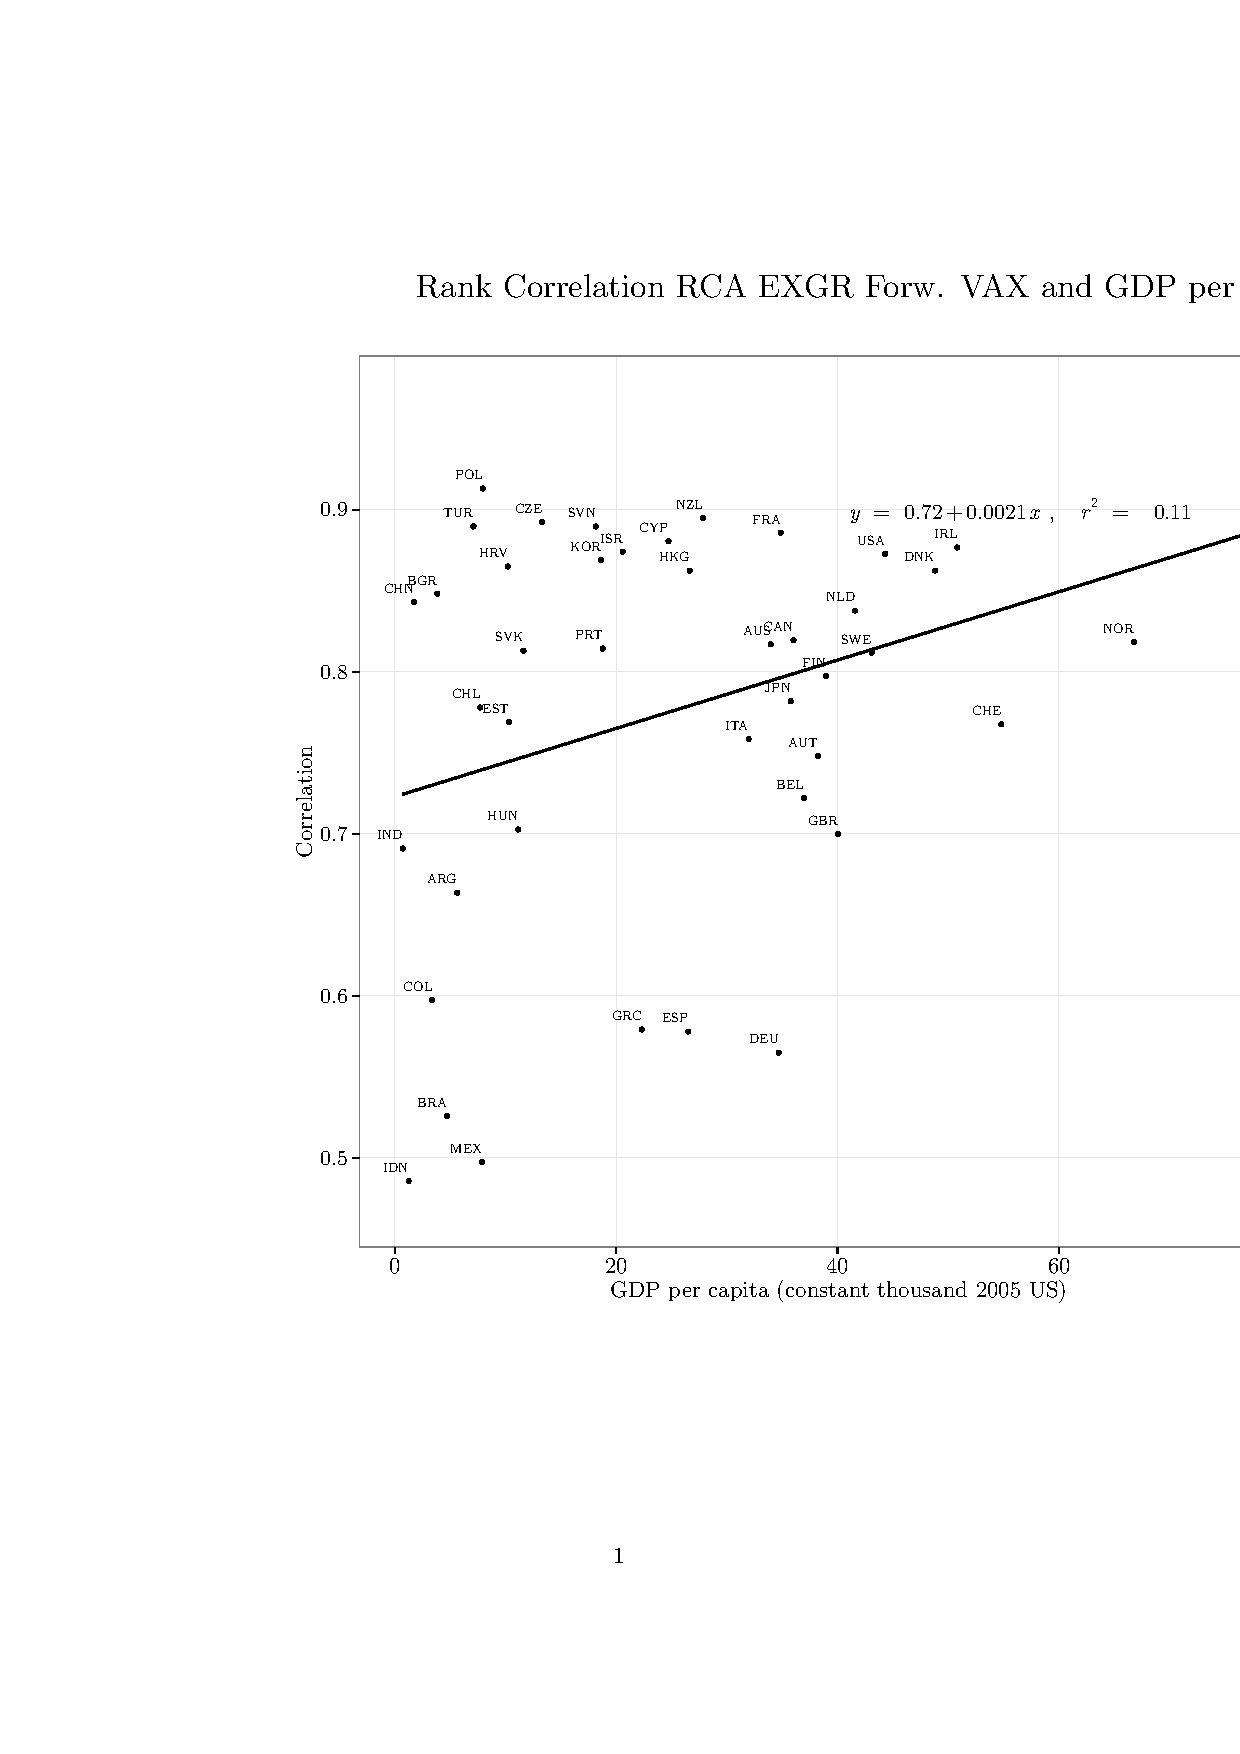
\includegraphics[width=.49 \linewidth]{./fig/spearman_fddva_std_balassa-march.tex}
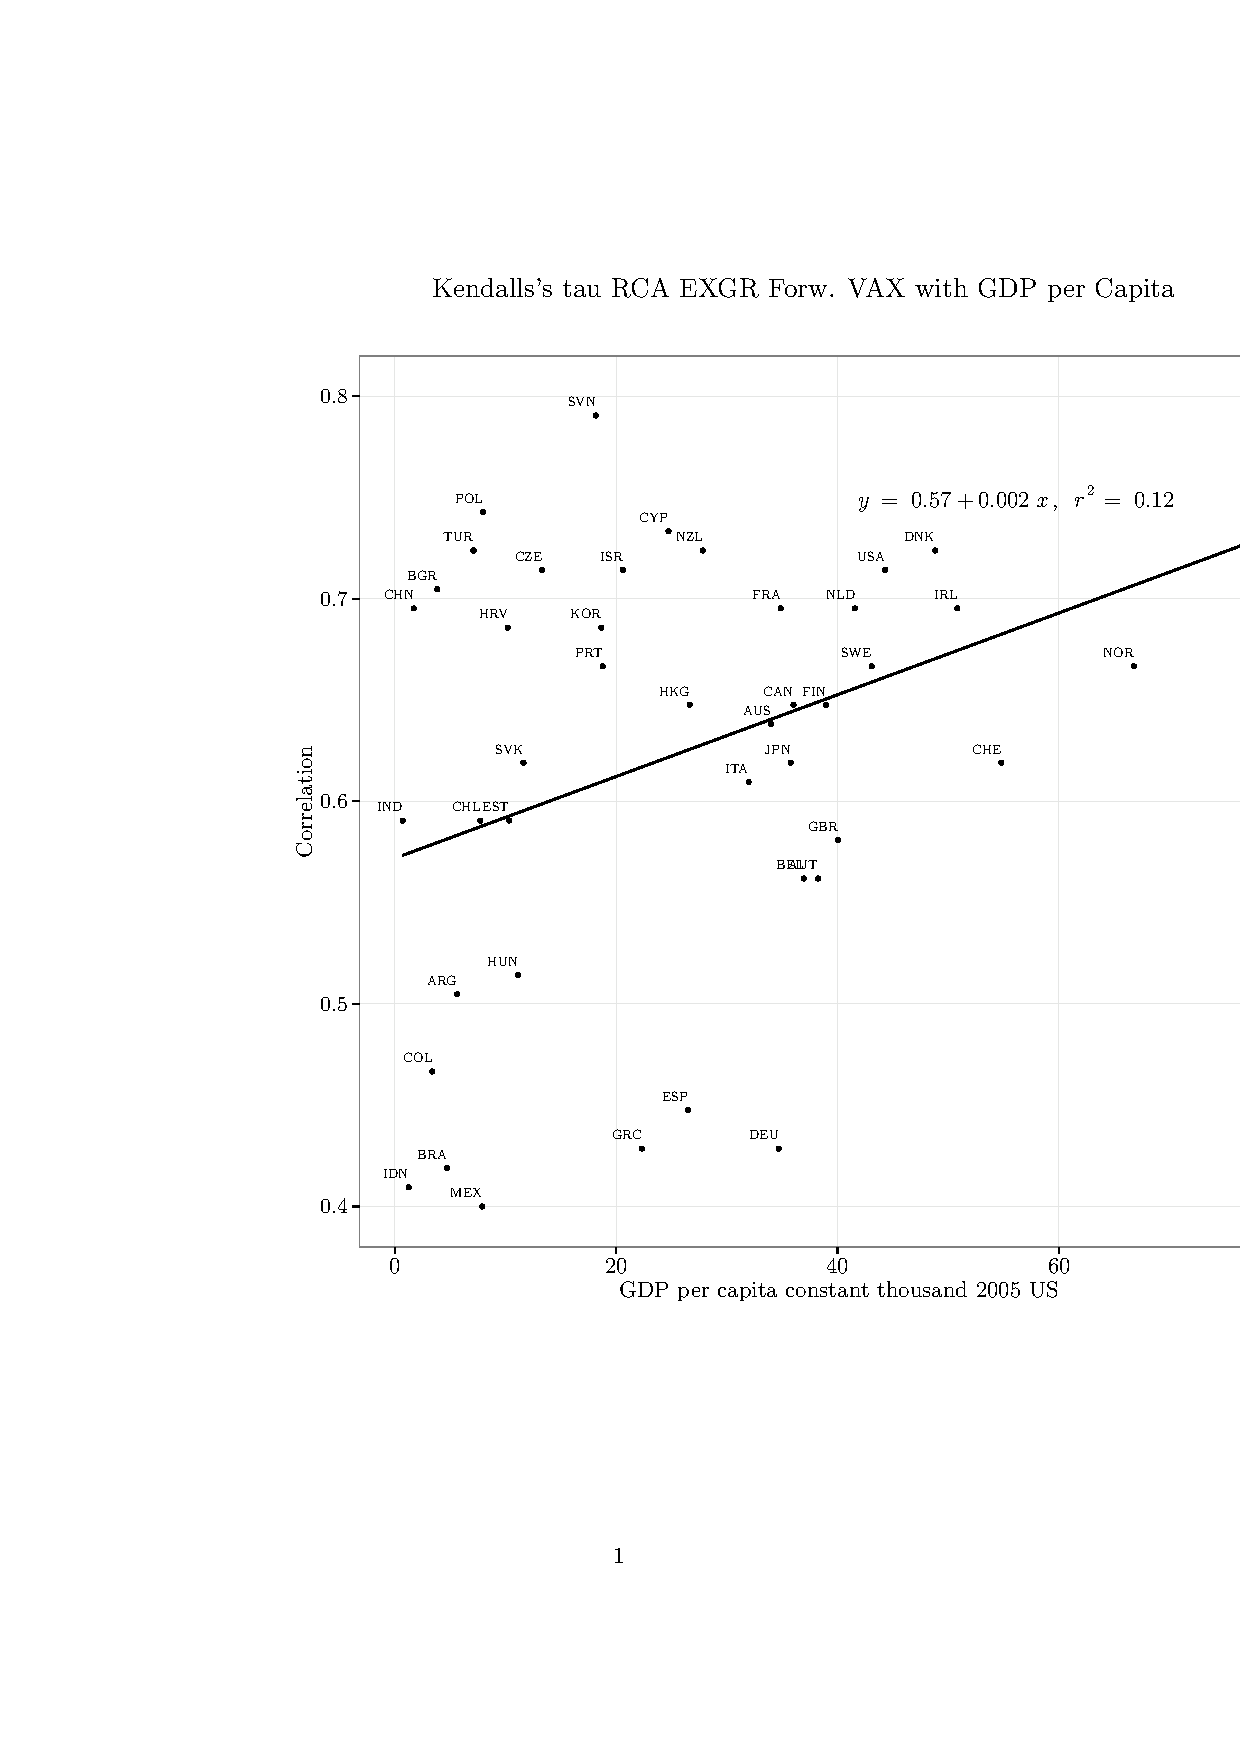
\includegraphics[width=.49\linewidth]{./fig/kendall_fddva_exgr_std_balassa-march.tex}
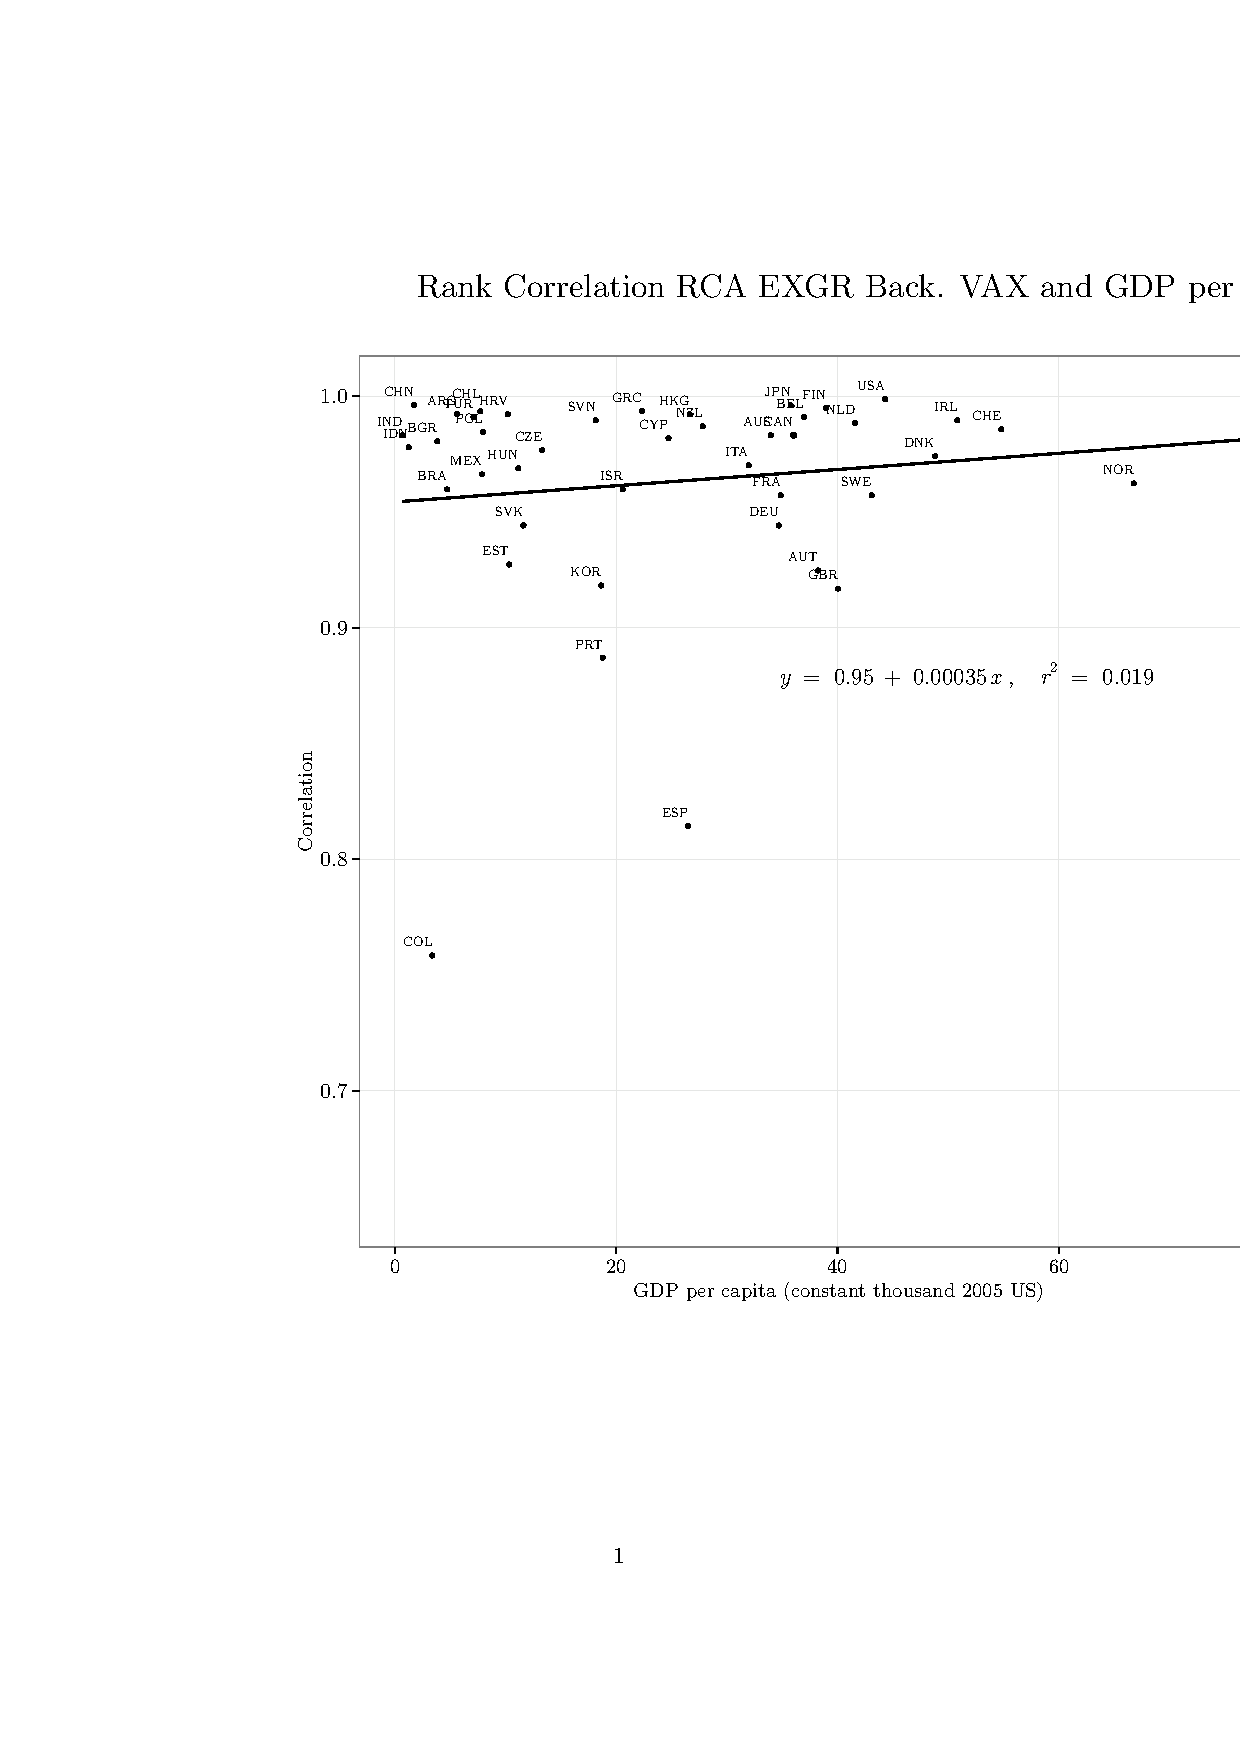
\includegraphics[width=.49 \linewidth]{./fig/spearman_exgr_dva_std_balassa-march.tex}
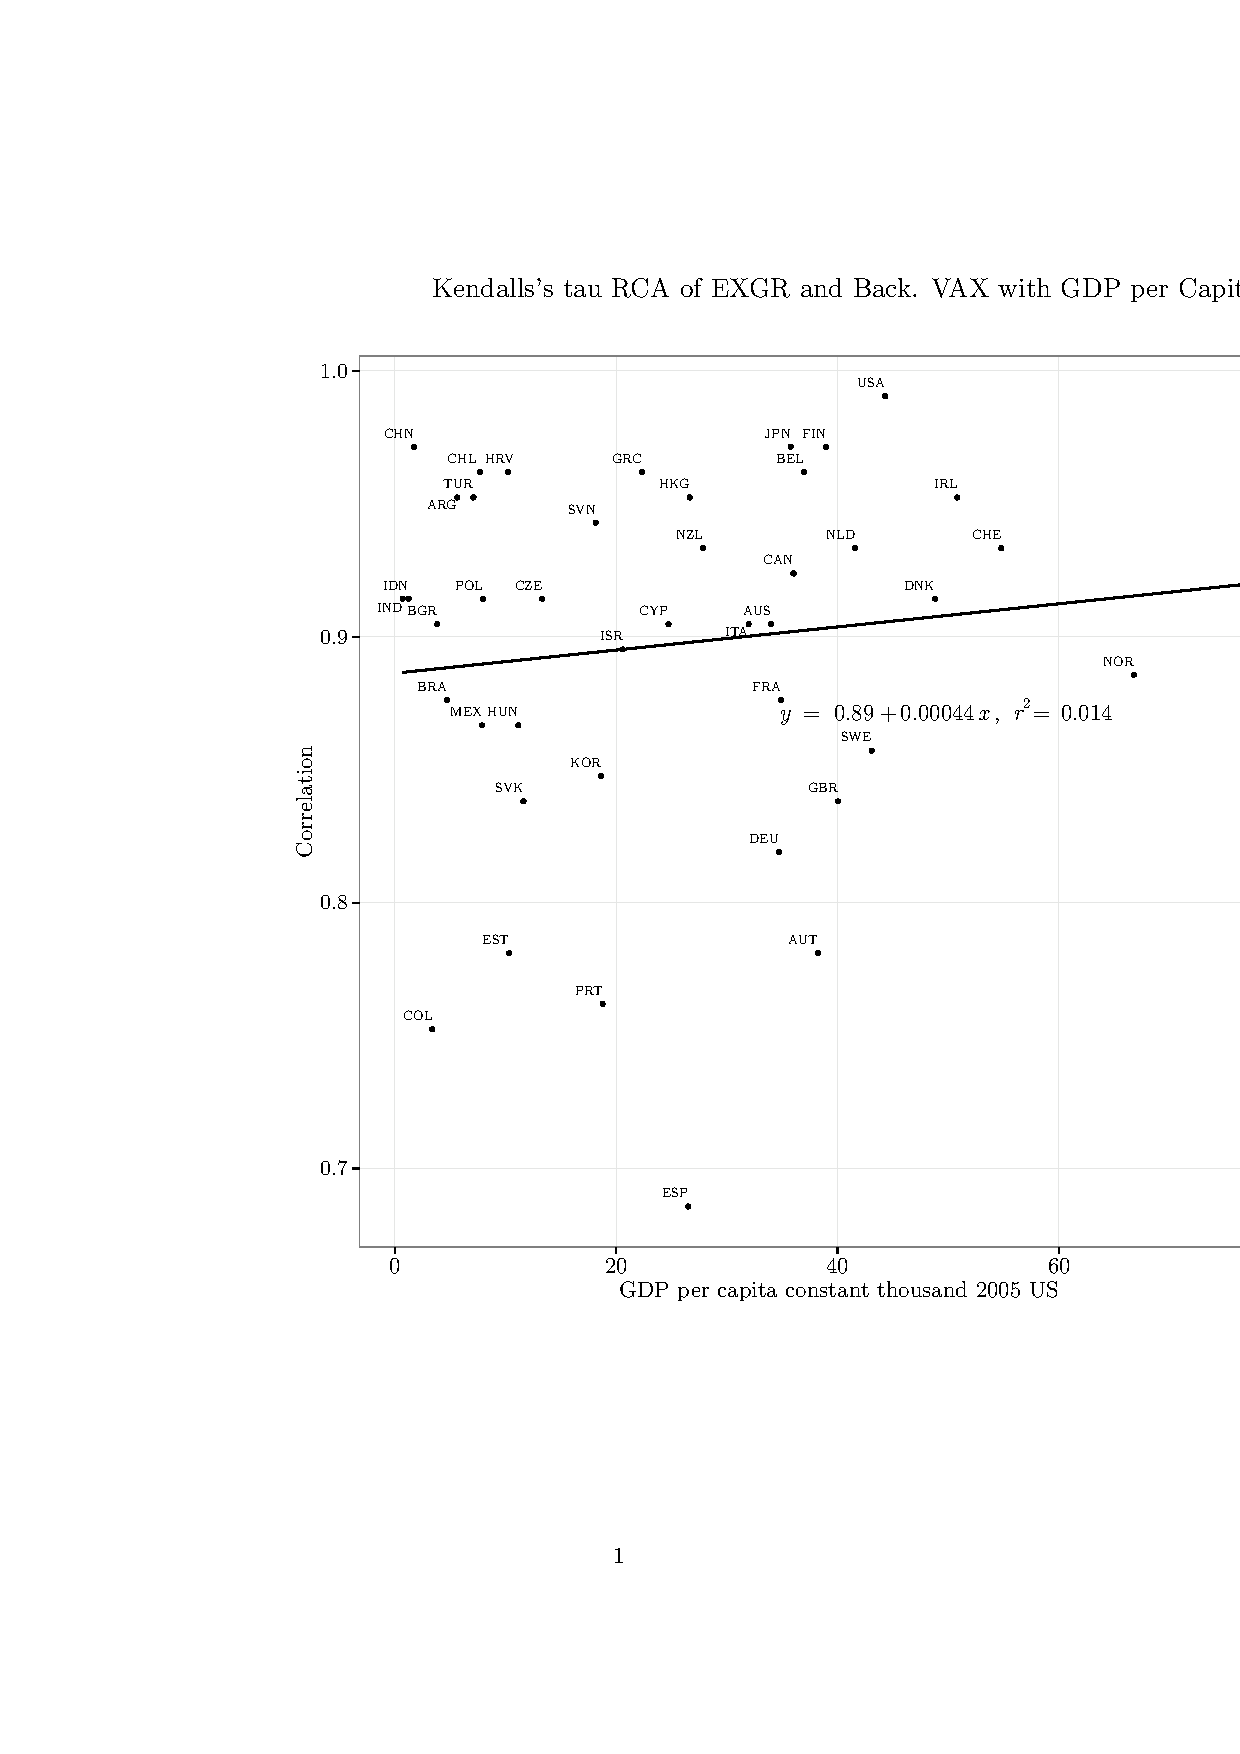
\includegraphics[width=.49\linewidth]{./fig/kendall_dva_exgr_std_balassa-march.tex}
 %\captionof{figure}{Another figure}
\end{figure}
I conclude four findings from the figures above.
Firstly, the RCA rankings based on gross exports and backward value-added exports show a high degree of similarity for all countries.
Secondly, the association between forward value-added exports and gross exports is substantially lower than the association of backward value-added and gross exports.
Thirdly,  the association of gross exports and forw. VAX show a weak positive association with a country's GDP per capita.
However the positive relation in the graph is not robust, as the exclusion of the country with the lowest and the highest  .
As a final point I find that the overall strength of the associations is higher using  Spearman's $\rho$ compared to Kendall's $\tau$. \par
The first and second finding are similar to the results in the estimation of the $\theta$ parameter, which showed similar estimates using gross exports and backward value-added exports while the estimates using forw. VAX showed differences.
The third finding is consistent with the hypothesis   that countries with a higher GDP have less sector specific input and sourcing patterns.
The finding of a smaller association for Kendall compared to Spearman is unsprising, given that the population analog of Spearman's $\rho$ and Kendall's $\tau$ is equal to three half \parencite{fredricks2007}. \par
The country pair graph comparing RCA for the three indicators backward/forward value-added exports and gross exports present a more local view of RCA.
 below I present  the normalized RCA based on both value-added export measures and gross exports for the industries of the manufacturing sector.
the RCA \footnote{ Formally, I define it as follows $RCA_{i}^{k}=\frac{ z^k_i * \bar{z} }{\bar{z}_i * \bar{z}^k}$, where $\bar{z}=1/NK* \sum_{i=1}^N \sum_{k=1}^K z^k_i$ denotes the grand mean, $\bar{z}^k= 1/N \sum_{i=1}^N z^k_i$ denotes the industry specific mean and $\bar{z}_i= 1/K \sum_{k=1}^K z^k_i$ denotes the country specific mean.} as in \textcite{leromain2014}.
The normalized RCA has the following interpretation, a value above (below) 1 indicates a comparative (dis)advantage of a country in a specific industry.
 \par
To start with the RCA ranking results, I discuss the results for backward value-added exports and gross exports.
I find that for both countries backward value added closely traces the RCA pattern of gross exports.
This results resembles the result of the estimation of $\theta$, where I observed a similar pattern. \par
The graph highlights that both countries highlights have an comparative advantage in the following sectors 20 23 24 26.
Germany has an higher comparative advantage in seven industries namely 20 21-22 25 27-28 29 30-33 34-35.
On the other hand, Belgium has an comparative advantage in six industries namely the food industry, 17-19 23 24 26 36-37.
 \par
In contrast, I observe that the RCA rankings are different for forward value-added gross exports.
The largest decrease of RCA based on forw. value-added exports compared to gross exports is in the industries 23 and 20.
Additionally for Germany large decrease of RCA for the industry 21-22.
The largest decrease of RCA induces a change of 15\%  in the industry 23 for both countries.
As a result, the industry 23 changes from a comparative advantage to a comparative disadvantage for Germany.
The industry changes from an comparative advantage to comparative disadvantage, whereas for Belgium the industry remains a comparative advantage.
Additionally, in industry 20 both countries show no longer an comparative advantage under forw. VAX, whereas under gross exports they show an comparative advantage.
Moreover, I observe the largest increase of RCA under VAX compared to EXGR in the industry 29 and 30-33.
For both countries I observe an increase of about 5\% in the industry 30-33 for forw. VAX, and a somewhat smaller increase in the industry 29.
However, the pattern of RCA remains unchanged for both countries, for Belgium an comparative disadvantage and Germany has an comparative advantage.
Concluding, the graphs show that forward value-added exports changes the pattern of RCA, whereas backward value-added exports traces the pattern of RCA under gross exports.
 \begin{figure}
\caption{Country pair RCA based on for- and backward  VAX \& EXGR }
\includegraphics[width=.5\linewidth]{./fig/forw_exgr_DEU_BEL_tiva.tex}
\includegraphics[width=.5\linewidth]{./fig/back_exgr_DEU_BEL_tiva.tex}
\end{figure}

\subsection{RCA based on WIOD}
In this subsection I compare the previous results about the RCA for BEL and GER to the results based on the WIOD data.
Firstly, compared to the TiVA data the WIOD data comes at a greater level of dissagregation.
\begin{figure}
\caption{Country pair RCA based on for- and backward  VAX \& EXGR }
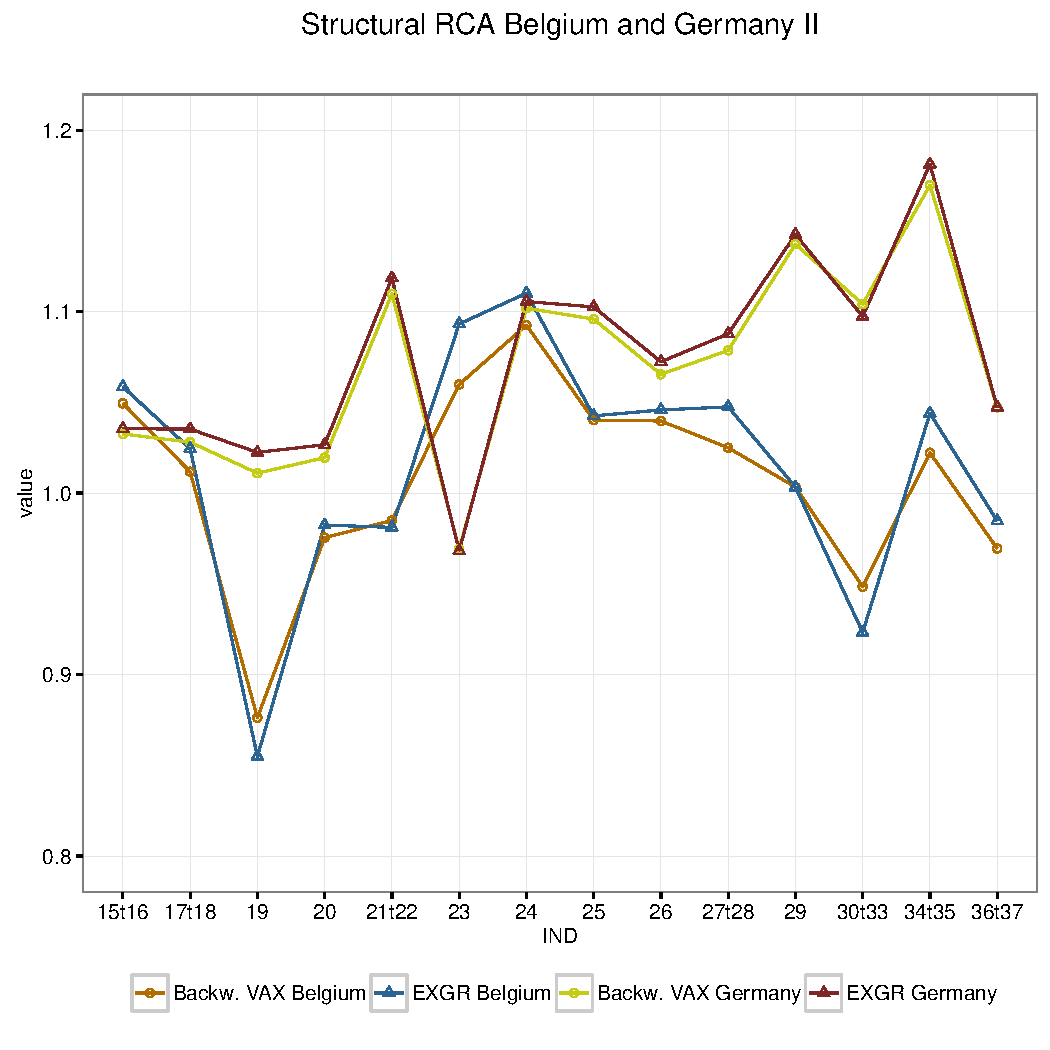
\includegraphics[width=.5\linewidth]{./fig/back_exgr_DEU_BEL_wiod.pdf}
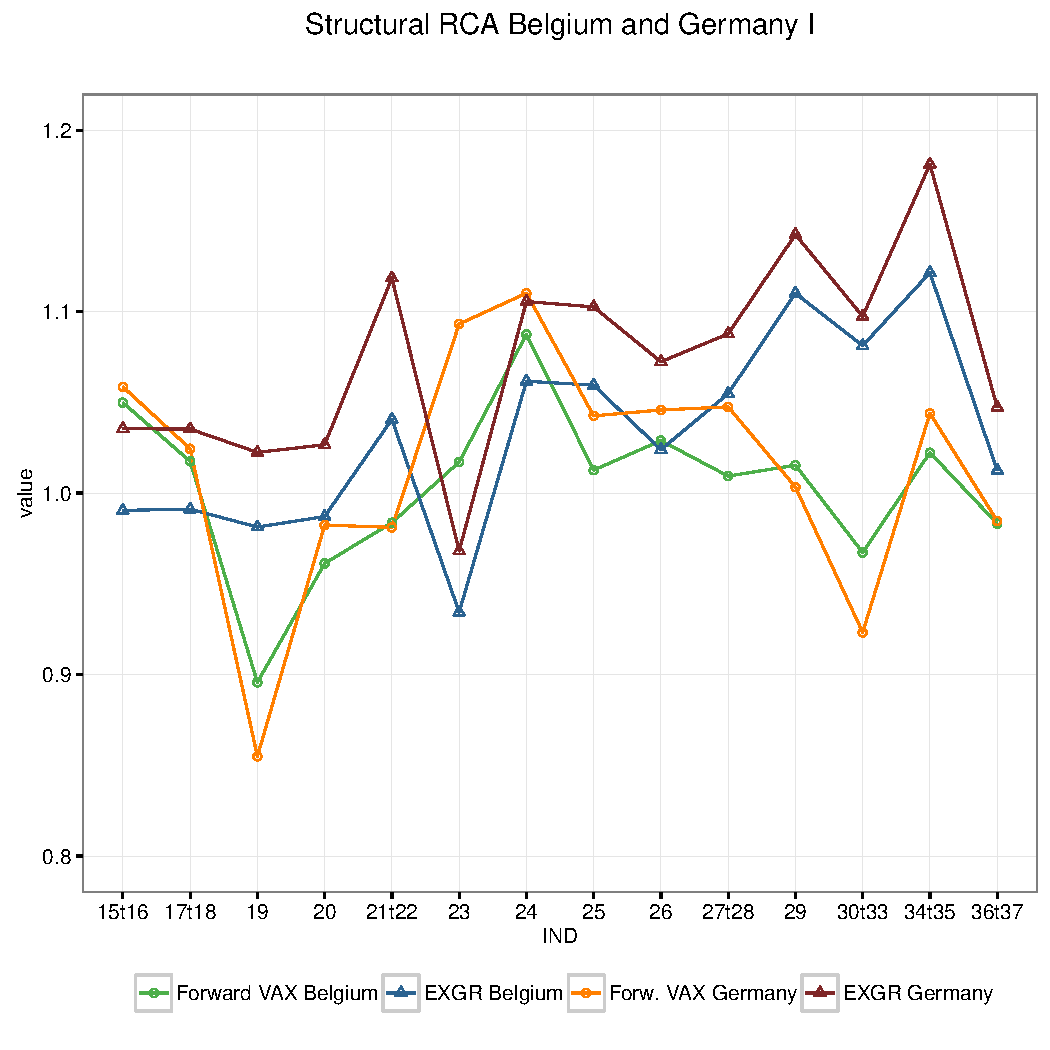
\includegraphics[width=.5\linewidth]{./fig/forw_exgr_DEU_BEL_wiod.pdf}
\end{figure}
\endinput

%!TEX root=root=C:/Users/Sergej/Documents/GitHub/Thesis/main.tex
\chapter{Relative network centrality and structural Ricardian comparative advantage}
%%Rajski?s information indices
In this chapter, I analyze the association between structural RCA  and network centrality.
 The motivation is as follows.
First according to Ricardo model  I expect that a industry within a country with relative lower cost to produce and export more a good.
The eigenvector centrality  of a country is high in a industry network if it exports to destinations which are important exporters themselves.
 A higher centrality of a country corresponds to higher trade shares.
 Therefore, we hypothesize that there may be a link between both measures. \\
The literature propagation of shocks in network  \cite{acemoglu2012} showed that network centrality
%why do we care
%similarity of network centrality to predictions of micro Ricardo model.
% Lower realtive cost to produce a good, hence higher trade shares.
%Eigenvector centrality by definition relative higher if I export to more important exporting countries.
% Acemolgu et al showed for the input output structure of an economy that industries with a higher network centrality conriubte more to a countrys GDP.
%Further they highlighted that network centrality is related to micro shocks.
% If the ranking of relative cost advantage is similar to network centrality, the latter is a simpler measure.
Further, I analyze the robustness of the results to changes of the normalization and  changes of the sample.
\section{International trade network}
In the following I define the trade network as directed and weighted network.
 The definition is based on \textcite{jackson2010} and \textcite{de2010}. I proceed by first defining the binary directed trade network and next the weighted trade network.\par
I define for each industry $k$ a trade network of $N = 1, \dots , n$ exporting countries $i$  and $N$ importing countries $j$.
The countries in the network are the nodes.
Each edge $g_{i,j}^k $ represents a trade relationship between an exporting industry $k$ in country $i$ and importing country $j$.
Since the trade relationships in each trade network are not symmetric the trade network is a directed network.
 \par
Specifically, I define a trade relationship as positive exports from industry $k$ in country $i$ to country $j$.
Each edge is represented by $g_{i,j}^k$, which is equal to one if there are positive exports in industry $k$ in country $i$ to country $j$ and zero otherwise.
Thus,
$g_{i,j}^k = \begin{cases}
 1 \quad \text{if} \quad x_{i,j}^k \neq 0 \\
0 \quad \text{if} \quad x_{i,j}^k = 0 \end{cases} $
For each industry $k$ the edges $g_{i,j}^k$ are recorded in a symmetric matrix  $g^k$  of the dimensions $n \times n$.
Now, based on the notation I define the binary trade network for each industry $k$ as the tuple of nodes and trade relationships $\cG^k(N, g^k)$. \par
To extent the binary trade network to its weighted version, I define the
weight variable $W_{i,j}^k$ which records the value of exports from industry $k$  in country $i$ to country $j$.
The weight of an edge  is thus denoted as the value of the exports in the trade relationship.
Analog to the matrices of trade relationships for the binary trade networks, I define for each industry $k$ a matrix, which records the weight of each trade relationship.
  This matrix $W^k$ is denoted as weight matrix. %Further, it has the interpretation of recording  the equilibrium relations at


er interactions have taken place \parencite{de2010}. \par
Based on the notation the weighted trade network for each industry is combination of the binary trade network and the weight matrix  $ITN^k =( \cG^k(N, g^k),W^k)$.
 \section{Network centrality}
The outline of eigenvector network centrality is based on the textbook of \textcite{jackson2010}, who attributes the original mathematical exposition to \textcite{Bonacich77}.
I first describe eigenvector centrality for a binary trade network.
The concept extends without modifications to a directed weighted network  \parencite{jackson2010}.  \par
Intuitively, eigenvector centrality describes the idea that a node is more central if it is connected to other central nodes.
The centrality of the other nodes is in turn determined by the centrality of the nodes are they are connected to.
Mathematically, defining the eigenvector centrality $C^e_i (g^k)$ associated with the network $g^k$, the centrality of an actor is proportional to the centrality of the nodes it is connected to.
\[  \lambda C^e_i (g^k) = \sum_{j \neq i}  g^k_{i,j}C^e_{i,j}(g^k)  \]
, where $\lambda$ is a proportionality constant.
Restating the equation in matrix notation and solving it
\begin{align*}
 \lambda C^e (g^k) & =  g^k C^e (g^k) \\
( I  \lambda-g^k) C^e(g^k) & = 0
 \end{align*}
where $ \lambda$ is the corresponding eigenvalue to the eigenvector $C^e(g^k)$.
In general this equation has $n$ solutions, however it is a convention to use the eigenvector corresponding to the largest eigenvalue.
An important property of the eigenvector is implied by the Perron-Frobenius theorem.
It states that for a non-negative column stochastic matrix
 \footnote{A column stochastic matrix is a matrix, where each column sum is equal to one.}, the right-hand eigenvector corresponding to the largest eigenvalue is positive
 and equivalently for a non-negative row stochastic matrix that the left hand  eignevector for the largest eigenvalue is positive.
Further, the theorem implies that if for some power the matrix $g^k$ is positive, than the largest eigenvalue is equal to one and all other eigenvalues are smaller.
 \par
Extending the eigenvector centrality concept to the weighted and directed trade network is straightforward.
Instead of computing the eigenvector for each adjacency matrix $g^k$, I calculate it for each weight matrix $W^k$.
Moreover, take advantage of the Peron-Frobenius Theorem I row-normalize the weight matrix, so that each cell is divided by the sum of exports of a country.
Each cell of the matrix thus records the share of exports of the country in the exporting industry across destinations. \par
In the steps I outlined to construct, I described the weighted out eigenvector centrality.
However, likewise one could instead of column normalize the weight matrix and obtain the left eigenvector, which is the in eigenvector centrality.
 \par
My analysis is based on the out eigenvector, due to the following consideration.
The out eigenvector centrality is computed for the row-normalized matrix, where each cell records the export shares.
A higher out centrality denotes that a country is exporting to countries with relative higher export shares.
On the other hand, the in-eigenvector a higher centrality would describe that a country is importing from countries with high shares of imports.
Therefore, I focus on the  out-eignevector centrality due to its similarity to the structural RCA.


%Moreover I highlighted in the introduction that the literature on shock propagation in networks, offers an interpretation of network centrality as a measure of ability to produce goods.  In the trade network I describe here, hence the network centrality describe the ability of an industry in a certain country.  \par The TiVA indicator as I described in section 2. describes the break down of domestic value-added sold across destinations
%Therefore for the network centrality I expect that industries, which are more central, contribute more to the value added sold across destinations. Further, if my interpretation of network centrality is correct, it should be the case that the relative centrality may be interpreted as measure of the relative ability to of an industry in some country to export relative to a benchmark industry and country. Therefore  I hypothesize that the ranking of relative centrality is similar to the ranking I obtain from the structural RCA measure.
\section{Network centrality and structural Ricardian comparative advantage}
In this subsection, I analyze the association between relative network centrality and  structural RCA based on domestic value added export.
I applied two normalizations to the eigenvector centrality as to the RCA before computing the association between them.
Firstly, I normalized  both measures to the grand mean, the mean across industries and the mean across countries.
Secondly, I normalized both measures relative to a benchmark country (the USA) and a benchmark industry (the food and beverages industry). \par
In the introduction I  outlined the similarity of out eigenvector centrality and the RCA.
Given the similarity, if structural RCA and network centrality show comparable results, the later may be preferred as a simpler measure.
% Network centrality by definition an industry is more central if the industry exports to relative more important central nodes.
%Moreover, according to the Ricardo model higher trade shares reflects a relative high productivity.
Additionally, the network shock propagation literature showed two aspects about network centrality,
Firstly, a industry with higher network centrality in the input-output network contributes relative more to the value-added.
 Moreover, it showed that network centrality is related to microshocks.
  \par
%In the introduction I hypothesized based on the network shock propagation literature,
%that interpret network centrality may be interpreted as a measure of ability of an industry.
%Moreover, the empirical heterogeneous firms literature found that firms with a higher ability to produce goods are more likely to export (\cite{bernard2007}, \cite{ottaviano}), which is in line with results of the theoretical heterogeneous firms literature  (\cite{bernard2003}, \cite{melitz}).
In the following I first describe Tthe left graph, which shows the association between network centrality and RCA according to the first normalization.
First interpreting the left graph I see that for most countries the association of the rankings are quite high.
This can be seen as the average of Spearman $/rho$ is  0.76 and Kendall's  $/tau$ is 0.58.
Both China and the USA have a high similarity between the rankings.
On the other hand Finland and Mexico show relative high dissimilarity between the rankings.
I obtain very strong results for India and Indonesia.
For India is that Spearmans $/rho$ and  Kendall's  $/tau$ are negative.
For Indonesia, the results show a low yet positive coefficients for both measures.
\par
The right graph shows overall a higher association between RCA and network centrality.
 This can be seen from the fact that the average of Spearman $/rho$ is  0.85 and Kendall's  $/tau$ is 0.71.
Like before the graph shows that India and Indonesia have the lowest similarity between both measures.
However, the strength of association for India is slightly increased so that the sign of the association is positive.
Both Finland and Mexico show a increased similarity in the graph.
Further, it is noteworthy that for Canada the strenght of both association is reduced, indicating that the
rankings differ more for Canada. \par
 Overall, the results suggest that the ranking of RCA and network centrality are similar for backward value-added exports.
  However, noteworthy for India and Indonesia I observed that both rankings are very different.
  Hence, future research should analyse the conection between RCA and network centrality from a theoretical perspective.

 \begin{figure}[H]
  \centering
\includegraphics[width=.45 \linewidth]{./fig/kend_spear_RCA_cent_april_i.tex}
\includegraphics[width=.45 \linewidth]{./fig/kend_spear_RCA_cent_april_ii.tex}
\end{figure}
\endinput

% \section{Robustness}
% In this section, I examine the robustness of the correlation between the structural RCA and relative network centrality.
% The  robustness test encompass computing the (rank) correlation for a different year 1995, and two different samples.
% The first sample covers the same countries as the extended sample used to estimate the fixed effects regression, except of the Rest of the world.
% Moreover, in both samples I changed the normalization such that the reference country is the USA and the reference industry is the food industry.
% %Moreover, I examine the time stability of the relative network centrality ranking.
% \par
% In the table \cref{tab:productivity_centrality_without_row} in column (2) and (3) the person and spearman correlation coefficients for the sample with rest of the world and in the columns (4)-(9) I report the deviation of the simple correlation or rank correlation from the coefficients in the columns (2) and (3). Moreover, I highlighted changes larger than 0.1 in grey.  \par First, the table confirms the robustness of the conclusion that the association between relative network centrality and the indicator of structural RCA  is stronger for the rank correlation than for the simple correlation. Moreover it confirms   that the relation between both is rather monotone than linear.  \par In addition, the change of the year shows overall an increased  simple correlation coefficients. The changes are heterogeneous showing both increased coefficients mostly for the service industry and some decreased coefficients in the manufacturing industries (ISIC 15-37). The largest increase is in the social service industry and for the construction industry. The largest decrease is reported for the wood industry. The rank correlation shows less changes in comparison. The largest increases are in the food industry and real estate industry. Overall the robustness check qualitatively leaves the conclusions unaltered. \par The change of the normalization and exclusion of ROW from the sample in the columns (6) to (7) shows  only minor effects for both correlations.  I record only one larger change for the simple correlation coefficient for the metal industry. The robustness check thus confirms the previous conclusions. \par In the last two columns I report the results of changing the sample to include only those countries, which were present in the estimation of the dispersion parameter. Eight industries have strong positive increased coefficients.  The industry with the largest increase is the communication industry. Four industries show small decreased coefficients. The industry with the largest decrease is  the wood industry.  Overall the simple correlation coefficients show a modest increase of about 0.09 or in relative terms of 13 \%. \par The rank correlation coefficients show for sixteen industries decreased coefficients. The largest decrease is in the gastronomy industry and in the social services industry.  Overall the decrease is on average 0.04 and is more modest  than the average increase of the simple correlation coefficients.  In the smaller sample the difference between the simple and rank correlation is half the size compared to the difference in the largest sample with ROW in 2005.\par  To conclude, all robustness test confirmed the previous results about the association between structural RCA and relative network centrality.
% %Overall the table \cref{tab:productivity_centrality_without_row}, confirms that the correlations between structural RCA and relative network centrality ranking is robust to changes in the reference country. The Pearson correlation shows the difference between column one and three of the absolute magnitude from -.07 to 0.13. The differences in the Pearson correlation are greater than the Spearman correlation. The differences in the Spearman correlations between column 2 and 4 are between 0.0 and 0.04, highlighting the robustness of the results.  %strange paragraph
% \begin{table}[H]
% \footnotesize
% \centering
%   \resizebox{0.9\textwidth}{!}{\begin{minipage}{\textwidth}
% \caption{Correlation structural RCA and relative network centrality -- robustness to changes in time, normalization and sample coverages}
% \label{tab:productivity_centrality_without_row}
% \begin{tabular}{l*{8}{S}}
%   \toprule
%  &\multicolumn{2}{c}{with Rest of the world 2005}& \multicolumn{2}{c}{with Rest of the world 1995} & \multicolumn{2}{c}{without Rest of the World} & \multicolumn{2}{c}{estimation sample*} \\
%  ISIC & \multicolumn{1}{c}{Simple}&\multicolumn{1}{c}{Rank} & \multicolumn{1}{c}{Simple} &\multicolumn{1}{c}{Rank  }  & \multicolumn{1}{c}{Simple}  &\multicolumn{1}{c}{Rank } &\multicolumn{1}{c}{Simple}  &\multicolumn{1}{c}{Rank  } \\ \midrule
% 15-16	&	0.87	&	0.76	&	-0.01	&	0.10	&	0.01	&	0.00	&	0.03	&	0.07	\\
% 17-19	&	0.61	&	0.95	&	\cellcolor{lightgray}0.13	&	-0.05	&	0.03	&	-0.03	&	\cellcolor{lightgray}	0.17	&	-0.07	\\
% 20	&	0.74	&	0.88	&	-0.09	&	-0.08	&	-0.08	&	0.01	&	-0.04	&	0.07	\\
% 21-22	&	0.74	&	0.93		&	0.00	&	0.00	&	0.03	&	0.00	&	-0.01	&	-0.01	\\
% 23	&	0.75	&	0.78		&		\cellcolor{lightgray}-0.18	&	0.04	&	-0.03	&	0.00	&	0.10	&	0.03	\\
% 24	&	0.77	&	0.93	&	-0.09	&	0.00	&	-0.06	&	-0.01	&	0.10	&	-0.02	\\
% 25	&	0.71	&	0.95		&	0.07	&	-0.02	&	0.03	&	-0.01	&	\cellcolor{lightgray}	0.12	&	-0.05	\\
% 26	&	0.65	&	0.97	&		\cellcolor{lightgray} 0.15	&	-0.03	&	0.07	&	-0.02	&	\cellcolor{lightgray}	0.18	&	-0.03	\\
% 27-28	&	0.78	&	0.94	&	-0.02	&	-0.01	&	\cellcolor{lightgray}-0.13	&	-0.02	&	-0.02	&	-0.06	\\
% 29	&	0.73	&	0.96	&	-0.05	&	-0.02	&	-0.03	&	-0.03	&	0.10	&	-0.06	\\
% 30-33	&	0.66	&	0.94	&	0.03	&	0.00	&	0.02	&	0.01	&	0.10	&	-0.02	\\
% 34-35	&	0.70	&	0.93	&	0.01	&	-0.01	&	0.03	&	-0.02	&		\cellcolor{lightgray}0.12	&	-0.06	\\
% 36-37	&	0.61	&	0.90		&	\cellcolor{lightgray}	0.18	&	0.03	&	0.02	&	-0.04	&		\cellcolor{lightgray}0.15	&	0.03	\\
% 45	&	0.55	&	0.89	&		\cellcolor{lightgray} 0.21	&	0.00	&	0.06	&	-0.01	&	0.10	&	-0.07	\\
% 50-52	&	0.79	&	0.92	&	0.01	&	-0.01	&	0.02	&	-0.01	&	0.02	&	-0.04	\\
% 55	&	0.58	&	0.89&		\cellcolor{lightgray}0.16	&	-0.10	&	0.05	&	-0.01	&		\cellcolor{lightgray}0.20	&		\cellcolor{lightgray}-0.11	\\
% 60-64	&	0.66	&	0.87	&		\cellcolor{lightgray}0.13	&	0.01	&	0.02	&	-0.03	&		\cellcolor{lightgray}0.23	&	-0.04	\\
% 65-67	&	0.72	&	0.92	&	0.01	&	-0.01	&	0.01	&	-0.01	&	0.06	&	-0.05	\\
% 70-74	&	0.69	&	0.85	&	0.10	&	0.09	&	-0.01	&	-0.02	&	-0.03	&	-0.03	\\
% 75-95	&	0.51	&	0.85		&		\cellcolor{lightgray} 0.26	&	0.03	&	0.03	&	-0.03	&	\cellcolor{lightgray}0.19	&	\cellcolor{lightgray}	-0.18	\\ \midrule
% AVG	&	0.69	&	0.90&	0.05	&	0.00	&	0.00	&	-0.01	&	0.09	&	-0.04	\\
% median	&	0.70	&	0.92	&	0.05	&	0.00	&	-0.01	&	-0.01	&	0.08 &	-0.04	\\  \bottomrule
%  \multicolumn{9}{l}{*The estimation sample covers the same countries as in the estimation of the productivity dispersion parameter}\\
%    \multicolumn{9}{l}{Benchmark Industry ISIC Rev. 3 01-05 } \\
% \multicolumn{9}{l}{Benchmark Country Rest  of the World \&  United States of America}  \\
%    \multicolumn{9}{l}{Industries with an deviation > 0.1 compared to  column 1/2 are highlighted grey  } \\
%   \end{tabular}
%       \end{minipage}}
% \end{table}
%Further as a robustness test I report the correlations between structural RCA  and relative network centrality for the full sample and the sample including only countries, which were also present in the estimation sample. \par Overall the Spearman correlation coefficients show a slightly reduced correlation in the estimation sample compared to the full sample. The Pearson correlation results point in the opposite direction. They show mostly higher coefficients in the estimation sample. Therefore both correlations show more similar correlation coefficients in the estimation sample. \par The conclusion from the table \ref{tab:prod_cent} remain unaltered. The relation between both concepts is monotone rather than linear because the Spearman correlation coefficients are mostly higher than the Pearson correlation. Further, both concepts show a very high correlation.
%
%\begin{table}[H]
%\footnotesize
%\centering\caption{Correlation structural RCA and relative network centrality*  in 2005 with Rest of the World and the estimation sample**}
%\label{tab:productivity_centrality_estimation_sample}
%\begin{tabular}{l*{4}{c}}
%\toprule
%&  \multicolumn{2}{c}{with Rest of the world} &\multicolumn{2}{c}{Estimation Sample} \\ \\
% ISIC& Pearson & Spearman  & Pearson & Spearman \\
%  \midrule
%15-16 & 0.87 & 0.76 & 0.90 & 0.83 \\
%  17-19 & 0.61 & 0.95 & 0.79 & 0.89 \\
%  20 & 0.74 & 0.88 & 0.70 & 0.95 \\
%  21-22 & 0.74 & 0.93 & 0.72 & 0.91 \\
%  23 & 0.75 & 0.78 & 0.84 & 0.79 \\
%  24 & 0.77 & 0.93 & 0.87 & 0.92 \\
%  25 & 0.71 & 0.95 & 0.83 & 0.91 \\
%  26 & 0.65 & 0.97 & 0.83 & 0.94 \\
%  27-28 & 0.78 & 0.94 & 0.75 & 0.88 \\
%  29 & 0.73 & 0.96 & 0.83 & 0.90 \\
%  30-33 & 0.66 & 0.94 & 0.76 & 0.91 \\
%  34-35 & 0.70 & 0.93 & 0.82 & 0.87 \\
%  36-37 & 0.61 & 0.90 & 0.76 & 0.93 \\  % Diff: 15 % Diff 3
%  45 & 0.55 & 0.89 & 0.63 & 0.83 \\
%  50-52 & 0.79 & 0.92 & 0.81 & 0.88 \\
%  55 & 0.58 & 0.89 & 0.78 & 0.76 \\  % Diff: 20 % Diff 12
%  60-64 & 0.66 & 0.87 & 0.89 & 0.80 \\
%  65-67 & 0.72 & 0.92 & 0.75 & 0.88 \\
%  70-74 & 0.69 & 0.85 & 0.65 & 0.81 \\
%  75-95 & 0.51 & 0.85 & 0.67 & 0.67 \\  \midrule
%  AVG & 0.69 & 0.90 & 0.78 & 0.86 \\
%  median & 0.70 & 0.92 & 0.78 & 0.88 \\   \bottomrule
%  \multicolumn{5}{l}{*based on domestic valued added exports}\\
%  \multicolumn{5}{l}{**The estimation sample covers the same countries}\\
% \multicolumn{5}{l}{Ricardo estimation sample}\\
%    \multicolumn{5}{l}{Benchmark Industry ISIC Rev. 3 01-05 }\\
%\multicolumn{5}{l}{Benchmark Country Rest of the World \& USA}\\
%\end{tabular}
%\end{table}
%
%%
%%Further I examine the time stability of relative network centrality between 1995 and 2005 in the table \ref{tab:rel_centr_95_05}.  For most sectors  I find that the table shows a strong or very strong correlation. The Pearson correlation coefficient spans between 0.51 and 0.97 \par
%%The Pearson correlation coefficient is the lowest for the construction sector, whereas the Spearman correlation is the lowest for the fuel industry. Most differences between both correlation coefficients are small except for the construction and the mineral industry. Most industries show a higher Spearman  correlation coefficient compared to the Pearson correlation coefficient. The table shows a substantial relative increase of the Spearman correlation coefficient compared to the Pearson coefficient by 36 \% from 0.51 to 0.80 in the construction industry.   The results suggest that the network centrality in most industries shows stable time ranking property.
%%\begin{table}[H]
%%\footnotesize
%%\centering\caption{Correlation between relative centrality* in 1995 \& 2005 }
%%\label{tab:rel_centr_95_05}
%%\begin{tabular}{l*{4}{c}}
%%  \toprule
%%ISIC Code & Pearson  & Spearman& P-val Pearson & P-val Spearman \\
%%  \midrule
%%15-16 & 0.78 & 0.85 & 0.00 & 0.00 \\  %7
%%  17-19 & 0.92 & 0.94 & 0.00 & 0.00 \\ %2
%%  20 & 0.87 & 0.91 & 0.00 & 0.00 \\ %4
%%  21-22 & 0.90 & 0.92 & 0.00 & 0.00 \\ %2
%%  23 & 0.97 & 0.66 & 0.00 & 0.00 \\ %-21
%%  24 & 0.89 & 0.91 & 0.00 & 0.00 \\ %2
%%  25 & 0.98 & 0.94 & 0.00 & 0.00 \\ %-4
%%  26 & 0.75 & 0.93 & 0.00 & 0.00 \\ %18
%%  27-28 & 0.90 & 0.91 & 0.00 & 0.00 \\ %1
%%  29 & 0.90 & 0.94 & 0.00 & 0.00 \\ %4
%%  30-33 & 0.90 & 0.91 & 0.00 & 0.00 \\ %1
%%  34-35 & 0.86 & 0.90 & 0.00 & 0.00 \\ %4
%%  36-37 & 0.73 & 0.89 & 0.00 & 0.00 \\ %14
%%  45 & 0.51 & 0.80 & 0.00 & 0.00 \\ %39
%%  50-52 & 0.92 & 0.93 & 0.00 & 0.00 \\ %1
%%  55 & 0.80 & 0.85 & 0.00 & 0.00 \\ %5
%%  60-64 & 0.80 & 0.89 & 0.00 & 0.00 \\ %9
%%  65-67 & 0.95 & 0.86 & 0.00 & 0.00 \\ %-9
%%  70-74 & 0.77 & 0.85 & 0.00 & 0.00 \\ %8
%%  75-95 & 0.85 & 0.87 & 0.00 & 0.00 \\  \midrule
%%  AVG & 0.85 & 0.88 &   &   \\
%%   \bottomrule
%%     \multicolumn{5}{l}{*based on domestic valued added exports}\\
%%   \multicolumn{5}{l}{Benchmark Industry ISIC Rev. 3 01-05 Agriculture}\\
%%\multicolumn{5}{l}{Benchmark Country Rest of the World}\\
%%\end{tabular}
%%\end{table}
%In this section, I conducted several robustness checks to assess whether the high correlations for the revealed productivity based on different indicators and between revealed productivity and network centrality. Overall I conclude that the conclusions form the previous section are robust to the choice of the country coverage and changes in the normalization and the time. %Further examining the time stability I found that the  the ranking of network centrality shows in most industries a strong time stability.

%!TEX root=C:/Users/Sergej/Documents/GitHub/Thesis/main.tex
\chapter{Conclusion}
The objectives of this thesis were two-fold.
First, assess whether the impact of IPF on the production process is such that traditional export measures no longer provide a reliable picture of technological comparative advantage.
A second objective was to analyze the association between relative network centrality and technological comparative advantage.
The hypothesis was motivated by the similarity of the interpretation of network centrality as how important an industry in a country in the export network is regarding \$ to the stochastic interpretation of trade shares resulting from productivity draws. \par
To analyze technological comparative advantage, I used an structural RCA measure based on the methodology of\textcite{costinot}.
The authors developed a theoretically consistent measure in a setup with imperfect specialization, multiple industries, and multiple countries.
 I estimated the measure for both domestic value-added and gross exports and compared the results using simple and rank correlations. \par
I proceeded in two steps to construct the structural RCA.
 In a first step I estimated a regression of the log of bilateral trade flows on the log of observed productivity, the inverse of international prices, an exporter-importer fixed effect and an importer-industry pair fixed effect.
  For this regression, I created a sample combining international relative price data from the GGDC \textcite{Inklaar2012}, R\&D data from the ANBERD OECD database and gross exports and value-added data from the \textcite{tiva2}.
  In the second step, I regressed the log of bilateral trade flows on the full set of export-importer, importer-industry and export-industry fixed effects.
   For the second estimation, I used the complete TiVA sample with 56 countries.  \par
In the first regression, I obtained an estimate for $\theta$, which may be interpreted as the inverse of the productivity dispersion.
 Comparing the point estimates of the productivity dispersion parameter to the results in \textcite{eaton} and in \textcite{costinot},
 I find that my point estimates were at the upper bound of the 95 \% confidence interval of the first and my estimates were significantly higher than the results of the latter.
  Moreover, I found that the estimates of $\theta$ using value-added exports showed increased values.
   This results may be explained by the construction of domestic value-added, which are net of double counting, foreign value-added and domestically absorbed exports.
   The variance of Domestic value-added exports band compared to gross exports.
   If fewer variations of the regressand are explained by the same variations of the observed productivity regressor, the estimated inverse of productivity dispersion $\theta$ should be increased.  \par
 Further, to assess the robustness of the estimates I reestimate the regression in the multiplicative form with PPML methods, as suggested by \textcite{silva}.
  The  estimates of the dispersion parameter showed a statistical not significant decreased estimate compared to the log-linear specification.
  An explanation of the result is that in the levels specification there is more variation of the regressand and, therefore, the estimates decreased.
  The results confirmed that the estimated values are not sensitive to the sample or the estimation technique. \par
Comparing the results of the structural RCA with gross exports and domestic value-added exports, I found that the simple and rank correlation coefficients showed very high coefficients.
The result suggests that the sector-specific input and sourcing patterns are similar do not vary strongly across sectors and, therefore, cleaning gross exports of foreign value-added does not change the ranking significantly.
Moreover, I compared the ranking results for the real estate industry to the results of \textcite{Koopman}.
In contrast to the authors, I find that domestic value-added exports do not change the ranking significantly. \par
 The second objective of this thesis was to analyze the empirical relation between relative network centrality and structural RCA.
 In network propagation of shocks literature, it was shown that for a single layer production network that network centrality is a first-order characteristic of how many actors contribute in \$ terms to the network.
 This interpretation is similar to the stochastic interpretation of trade shares as a result of productivity draws.
   Hence,  I  analyzed the association between relative centrality and structural RCA.
   The results of a correlation analysis showed a stronger rank correlation than simple correlation and hence pointed out that the association is rather monotone than linear between both measures.
   In conclusion, the strong empirical correlation supports the hypothesis. \par
  A direction for future work is to establish a theoretical model that explains the strong association of relative network centrality of an industry in a country in the international production network and structural RCA.
  Moreover, future work may analyze the association between a RCA ranking based on domestic value-added exports and the ranking predicted by the Heckscher-Ohlin model.
\endinput

\clearpage
\printbibliography
\vfill
\pagestyle{empty}
\appendix
\sisetup{
	detect-mode,
		group-digits		= false,
		input-symbols		= ( ) [ ] - +,
		table-align-text-post	= false,
		input-signs             = ,
		        round-mode              = places,
        round-precision         = 2
 }


\tocless \chapter{Appendix}
\addcontentsline{toc}{chapter}{Appendix}
%!TEX root=/Users/sergej/Documents/Master/Thesis/main.tex 

\section{Decomposition of gross exports into value-added exports}
I use the indicators from the OECD-TiVA database later to compute the RCA ranking based on the two step method described in \textcite{costinot} and compare the  rankings to an RCA ranking based on gross exports.  
\par 
Input-Output tables are models of the economy based on the work of \textcite{leontief}. The intuitive insight of  Leontief was to record the usage of intermediate inputs and production factors to produce units of output in a matrix. He showed that the recursion  can be mathematically solved until one accounts for the complete set of intermediate inputs to produce one unit of output.  Leontief's insight of modeling input-output relations is sufficient to decompose gross exports into domestic value-added exports \parencite{Koopman}. \par
At this point, a note on the data limitations concerning Input-Output tables is necessary.  Ideally value-added exports data would be decomposed from global Input-Output tables provided by national statistical agencies. Yet, global input-output data do not exist, and therefore scientist and different international organizations construct synthetic global Input-Output tables based on National Input-Output tables \parencite{johnson}. \par 
In the following I will illustrate the decomposition of gross exports into forward and backward vale-added exports for two simple cases. Interested readers may be referred to the work of \textcite{Koopman} for a more general treatment.
%Next, I lay out the definition of domestic value-added exports. I define $x^k_{i,j}$  as gross exports from industry $k$ in exporting country $i$  to  importing country $j$. Further I decompose bilateral gross exports $x_{i,j}$ as the sum of  intermediate exports $I^k_{i,j}$ and exports to final demand $F^k_{i,j}$, thus  \[ x_{i,j}=\sum_k x^k_{i,j} =\sum_k (I^k_{i,j}+F^k_{i,j} )\]. In addition I define $V_i$ as a $K \times K$ matrix, which contains on the diagonal the domestic value-added shares from each industry $k$ in country $i$. 
%\[V_i=\left( \begin{matrix}
%    V_{i,1} & \ldots  &0 \\
%\vdots & \ddots& \vdots \\
%   0 & \ldots  & V_{i,k} 
%\end{matrix} \right)
%\]
% Further, I denote with  $B=(\mathcal{I}-A)^{-1}$ the global Leontief inverse with $NK \times NK$ dimensions, $A$  denotes the global Input-Output coefficient matrix and $\mathcal{I}$ denotes the identity matrix. \par 
% The Leontief inverse describes by how much one country's gross output increases if the final demand of another country increase by one unit \parencite{wang2013}. \par The Input-Output coefficient matrix describes the production technology. \par 
% Domestic value-added embodied in gross exports is therefore
% \[x^{DVA}_i=\sum_{j} x^{DVA}_{i,j} = \sum_{j} V_{i}B_{i,i}     x_{i,j}\]
%where the index $j$ denotes the partner country, $x^{DVA}_{i,j}$ denotes the $K \times 1$ vector denoting a country $i$'s domestic value-added embodied in gross exports to country $j$ for any industry $k$ and $B_{i,i}$ is the block diagonal matrix of $B$ of the dimensions $K \times K$.  \par
\section{ISIC and ISO 3 Alpha Classification}
\begin{table}[H]
\centering \caption{ISIC Revision 3.1}
\begin{tabular}{lll}
\toprule
ISIC Code&Short & TiVA Description \\ 
\midrule
  01-05  &Agriculture & Agriculture, hunting, forestry and fishing \\ 
10-14& Mining& Mining and quarrying \\ 
15-16& Food & Food products, beverages and tobacco \\ 
17-19&  Textiles& Textiles, textile products, leather and footwear \\ 
20& Wood & Wood and products of wood and cork \\ 
  21-22& Paper & Pulp, paper, paper products, printing and publishing \\ 
  23 &Fuel& Coke, refined petroleum products and nuclear fuel \\ 
  24 &Chemicals& Chemicals and chemical products \\ 
  25 &Plastic& Rubber and plastics products \\ 
  26&Minerals & Other non-metallic mineral products \\ 
  27-28&Metals & Basic metals and fabricated metal products \\ 
  29 &Machinery & Machinery and equipment, nec  \\ 
  30-33&Electrical & Electrical and optical equipment \\ 
  34-35 &Transport& Transport equipment \\ 
  36-37 &Misc. Manufacturing& Manufacturing nec; recycling  \\ 
  40-41 &Electricity & Electricity, gas and water supply \\ 
  45  & Construction& Construction \\ 
  50-52&Trade & Wholesale and retail trade; repairs \\ 
 55 &Gastronomy & Hotels and restaurants \\ 
  60-64&Communication & Transport and storage, post and telecommunication \\ 
  65-67 &Finance& Financial intermediation \\ 
  70-74 &Real estate& Real estate, renting and business activities \\ 
  75-95& Social & Community, social and personal services  \\ 
   \bottomrule
\end{tabular}
\end{table}

\begin{table}[H]
\footnotesize
\centering\caption{ISO 3 Alpha Code}
{
\def\sym#1{\ifmmode^{#1}\else\(^{#1}\)\fi}
\begin{longtable}{l*{1}{l}l*{1}{l}}
\toprule\endfirsthead\midrule\endhead\midrule\endfoot\endlastfoot
  COU             &\multicolumn{1}{c}{Country} &COU             &\multicolumn{1}{c}{Country}\\
\midrule
ARG             &     Argentina& ITA             &     Italy\\
AUS             &     Australia& JPN             &     Japan\\
AUT             &     Austria& KOR             &     Korea\\
BEL             &     Belgium& LTU             &     Lituhania\\
BGR             &     Bulgaria&LUX             &     Luxembourg\\
BRA             &     Brazil& LVA             &     Latvia\\
CAN             &     Canada& MEX             &     Mexico\\
CHE             &     Switzerland& MYS             &     Malaysia\\
CHL             &     Chile& NLD             &     Netherlands\\
CHN             &    China& NOR             &     Norway\\
COL             &     Colombia&  NZL             &     New Zeeland\\
CYP             &     Cyprus& PHL             &     Philippiens\\
CZE             &     Czech Republic& POL             &     Poland \\
DEU             &     Germany& PRT             &     Portugal\\
DNK             &     Denmark& ROU             &     Romania\\
ESP             &     Spain&  ROW             &     Rest of the World\\
EST             &     Estonia& RUS             &     Russian Federation\\
FIN             &     Finland& SGP             &     Singapore\\
FRA             &     France&  SVK             &     Slovakia\\
GBR             &     United Kingdom& SVN             &  Slovenia\\
GRC             &     Greece& SWE             &     Sweden\\
HKG             &     Hong Kong& THA             &     Thailand\\
HRV             &     Croatia& TUN             &     Tunisia\\
HUN             &     Hungary& TUR             &     Turkey\\
IDN             &     India& TWN             &     Taiwan\\
IND             &     Indonesia& USA             &    United States of America\\
IRL             &     Ireland& VNM             &     Vietnam\\
ISR             &     Israel& ZAF             &     South Africa\\ 
\bottomrule
\end{longtable}
}
\end{table}

\section{Data Appendix}
\subsection{Sample Statistics}

\begin{table}[H]\centering\caption{Summary statistics in estimation sample }
\footnotesize
\label{tab:sumstat}
\begin{adjustbox}{width=1\textwidth}
\begin{tabular}{l SSSSS}\toprule
\multicolumn{1}{c}{\textbf{Variable}} & \textbf{Mean}
 & \textbf{Std. Dev.}& \textbf{Min.} &  \textbf{Max.} & \textbf{N}\\ \midrule
Log Backward Value Added Exports&  2.443 & -4.60517  & 10.75376&2.867  & 17453\\
Log Gross Exports & 2.742 & 2.871  & - 4.60517  & 11.10807& 17505\\
Log Forward Value-Added Exports& 3 & 2.351 & - 4.605 & 10.739 & 15999\\
Log Productivity & .2664933 &   .2741434&  -.6715387  & 1.166582 & 18444\\
Log R\&D & 17.80132 &   2.441721 &  10.74497   & 24.7591 & 17313\\
\bottomrule
\end{tabular}
\end{adjustbox}
\end{table}
%\begin{table}[h]\centering\caption{Pairwise Correlation in estimation sample }
%\footnotesize
%\label{tab:pwcorr}
%\scalebox{0.85}{
%{
%\def\sym#1{\ifmmode^{#1}\else\(^{#1}\)\fi}
%\begin{tabular}{l*{4}{c}}
%\toprule
%          &\multicolumn{1}{c}{(1)}&\multicolumn{1}{c}{(2)}&\multicolumn{1}{c}{(3)}&\multicolumn{1}{c}{(4)}\\
%          &\multicolumn{1}{c}{log gross exports}&\multicolumn{1}{c}{log of productivity}&\multicolumn{1}{c}{log R \&D expenditures}&\multicolumn{1}{c}{log domestic value-added exports}\\
%\midrule
%log gross exports&                     &  -0.0921\sym{***}&    0.434\sym{***} & 0.996\sym{***}\\
%
%log of productivity&  -0.0921\sym{***}&                  &   -0.200\sym{***} &  -0.0996\sym{***}\\
%
%log R\&D expenditures &    0.434\sym{***}&   -0.200\sym{***}&              &    0.446\sym{***}    \\
%
%log domestic value-added exports&          0.434 &	0.446&	0.488	-0.200	1.000	
%\\
%\bottomrule
%\multicolumn{5}{l}{\footnotesize \sym{*} \(p<0.05\), \sym{**} \(p<0.01\), \sym{***} \(p<0.001\)}\\
%\end{tabular}
%}
%}\end{table}
\begin{table}[H]
\centering\caption{Pairwise correlation in estimation sample }
\footnotesize
\label{tab:pwcorr}
\scalebox{0.8}{
{
\def\sym#1{\ifmmode^{#1}\else\(^{#1}\)\fi}
\begin{tabular}{lSSSSS}\toprule
\multicolumn{1}{c}{Variables} &\multicolumn{1}{c}{Log gross exports}&\multicolumn{1}{c}{Log backward value-added exports}&\multicolumn{1}{c}{ Log forward value-added exports}&\multicolumn{1}{c}{Log Productivity}&\multicolumn{1}{c}{Log R\& D}\\ \midrule
Log gross exports								 &1.000 &   		& 		  &				&   \\
Log backward value-added exports &0.996&1.000 & 		  &				&    \\
Log forward value-added exports   &0.872&0.890&1.000 & 				&     \\
Log productivity									&-0.092&-0.100&-0.211&1.000& 		\\
log R\&D 												&0.434&0.446&0.488&-0.200&1.000\\
\bottomrule
%\multicolumn{5}{l}{\footnotesize \sym{*} \(p<0.05\), \sym{**} \(p<0.01\), \sym{***} \(p<0.001\)}\\
\end{tabular}
}
}
\end{table}

\begin{table}[H]
\footnotesize
\centering\caption{N. obs / IND  in estimation sample}
{
\def\sym#1{\ifmmode^{#1}\else\(^{#1}\)\fi}
\begin{longtable}{l*{1}{c} l*{1}{c}}
\toprule\endfirsthead\midrule\endhead\midrule\endfoot\endlastfoot
          \multicolumn{1}{c}{IND}          &\multicolumn{1}{c}{N}       &    \multicolumn{1}{c}{IND}          &\multicolumn{1}{c}{N}\\
\midrule
01-05       &         841      &
10-14       &         841         \\
\addlinespace
15-16       &         841      &
17-19       &         841         \\
\addlinespace
20          &         841      &
21-22       &         841         \\
\addlinespace
23          &         841      &
24          &         841         \\

\addlinespace
25          &         841      &
26          &         841         \\

\addlinespace
27-28       &         841      &
29          &         841         \\

\addlinespace
30-33       &         841      &
34-35       &         841         \\

\addlinespace
36-37       &         841      &
45          &         841         \\

\addlinespace
50-52       &         841      &
55          &         841         \\

\addlinespace
60-64       &         841      &
65-67       &         841         \\

\addlinespace
70-74       &         841      &
75-95       &         841         \\

\addlinespace
Total       &       18502         \\

\midrule
\bottomrule
\end{longtable}
}
\end{table}
\begin{table}[H]
\footnotesize
\centering \caption{N. obs /  COU in  estimation   sample }
{
\def\sym#1{\ifmmode^{#1}\else\(^{#1}\)\fi}
\begin{longtable}{l*{1}{c}l*{1}{c}}
\toprule\endfirsthead\midrule\endhead\midrule\endfoot\endlastfoot
   COU             &\multicolumn{1}{c}{N}&  COU             &\multicolumn{1}{c}{N}\\
\midrule
AUS         &         572     &
AUT         &         572            \\ \addlinespace
BEL         &         572     &
CAN         &         572        \\ \addlinespace
CZE         &         572     &
DEU         &         572        \\ \addlinespace
ESP         &         572     &
EST         &         572        \\ \addlinespace
FIN         &         572     &
FRA         &         572        \\ \addlinespace
GBR         &         572     &
GRC         &         572        \\ \addlinespace
HUN         &         572     &
IRL         &         572        \\ \addlinespace
ITA         &         572     &
JPN         &         572        \\ \addlinespace
KOR         &         572     &
LUX         &         572        \\ \addlinespace
MEX         &         572     &
NLD         &         572        \\ \addlinespace
POL         &         572     &
PRT         &         572        \\ \addlinespace
SVK         &         572     &
SVN         &         572        \\ \addlinespace
TUR         &         572     &
USA         &         572        \\ \addlinespace
Total       &        \multicolumn{2}{c}{114872}         \\
\bottomrule
\end{longtable}
}
\end{table}

\begin{table}[H]
\footnotesize
\centering\caption{N. obs / COU in structural RCA sample}
{
\def\sym#1{\ifmmode^{#1}\else\(^{#1}\)\fi}
\begin{longtable}{l*{1}{c}l*{1}{c}}
\toprule\endfirsthead\midrule\endhead\midrule\endfoot\endlastfoot
  COU             &\multicolumn{1}{c}{N} &COU             &\multicolumn{1}{c}{N}\\
\midrule
\midrule
ARG         &         946        & 
AUS         &         946         \\
\addlinespace
AUT         &         946        & 
BEL         &         946         \\
\addlinespace
BGR         &         946        & 
BRA         &         946         \\
\addlinespace
CAN         &         946        & 
CHE         &         946         \\
\addlinespace
CHL         &         946        & 
CHN         &         946         \\
\addlinespace
COL         &         946        & 
CYP         &         946         \\
\addlinespace
CZE         &         946        & 
DEU         &         946         \\
\addlinespace
DNK         &         946        & 
ESP         &         946         \\
\addlinespace
EST         &         946        & 
FIN         &         946         \\
\addlinespace
FRA         &         946        & 
GBR         &         946         \\
\addlinespace
GRC         &         946        & 
HKG         &         946         \\
\addlinespace
HRV         &         946        & 
HUN         &         946         \\
\addlinespace
IDN         &         946        & 
IND         &         946         \\
\addlinespace
IRL         &         946        & 
ISR         &         946         \\
\addlinespace
ITA         &         946        & 
JPN         &         946         \\
\addlinespace
KOR         &         946        & 
LUX         &         946         \\
\addlinespace
MEX         &         946        & 
NLD         &         946         \\
\addlinespace
NOR         &         946        & 
NZL         &         946         \\
\addlinespace
POL         &         946        & 
PRT         &         946         \\
\addlinespace
SVK         &         946        & 
SVN         &         946         \\
\addlinespace
SWE         &         946        & 
TUR         &         946         \\
\addlinespace
USA         &         946        & 
Total       &       40678         \\
\bottomrule
\end{longtable}
}
\end{table}
\begin{table}[H]
\centering\caption{N. obs / IND in  structural RCA sample}
 {
\def\sym#1{\ifmmode^{#1}\else\(^{#1}\)\fi}
\begin{longtable}{l*{1}{c}l*{1}{c}}
\toprule\endfirsthead\midrule\endhead\midrule\endfoot\endlastfoot
          \multicolumn{1}{c}{IND}          &\multicolumn{1}{c}{N}& \multicolumn{1}{c}{IND}          &\multicolumn{1}{c}{N}\\
\midrule                  
01-05       &        1849       &
10-14       &        1849         \\
\addlinespace
15-16       &        1849       &
17-19       &        1849         \\
\addlinespace
20          &        1849       &
21-22       &        1849         \\
\addlinespace
23          &        1849       &
24          &        1849         \\
\addlinespace
25          &        1849       &
26          &        1849         \\
\addlinespace
27-28       &        1849       &
29          &        1849         \\
\addlinespace
30-33       &        1849       &
34-35       &        1849         \\
\addlinespace
36-37       &        1849       &
45          &        1849         \\
\addlinespace
50-52       &        1849       &
55          &        1849         \\
\addlinespace
60-64       &        1849       &
65-67       &        1849         \\
\addlinespace
70-74       &        1849       &
75-95       &        1849         \\
\addlinespace
Total       &       \multicolumn{2}{c}{40678 }        \\
\bottomrule
\end{longtable}
}
\end{table}

\subsection{First Stage}
\begin{table}[H]
\footnotesize
\def\sym#1{\ifmmode^{#1}\else\(^{#1}\)\fi}
\begin{tabular}{l*{3}{S}}
\toprule
            &\multicolumn{1}{c}{(1)}&\multicolumn{1}{c}{(2)}&\multicolumn{1}{c}{(3)}\\
            &\multicolumn{1}{c}{Full Sample}&\multicolumn{1}{c}{Without primary industries}&\multicolumn{1}{c}{Without primary industries $\text{high}^1$ } \\
\midrule
Log of R\&D  &      .0221331 \sym{***}&        .0225872   \sym{***}&       .0203635   \sym{***}\\
            &        (0.002)        &     (.0020154)         &     (.0022056)       \\
\midrule
Exporter Importer FE & \multicolumn{1}{c}{Yes} & \multicolumn{1}{c}{Yes}& \multicolumn{1}{c}{Yes}\\
Importer Industry FE & \multicolumn{1}{c}{Yes}& \multicolumn{1}{c}{Yes}& \multicolumn{1}{c}{Yes} \\
\(N\)       &     19343    &     17661    &         15283         \\
%\(R^{2}\)   &          0.614         &       0.645         &       0.693          \\
F (excluding dummies)    &     125.60         &      88.171         &    85.24         \\
Imputations & 29 & 29 & 29 \\
\bottomrule
\multicolumn{4}{l}{\footnotesize Standard errors in parentheses}\\
\multicolumn{4}{l}{\footnotesize \sym{*} \(p<0.05\), \sym{**} \(p<0.01\), \sym{***} \(p<0.001\)}\\
\end{tabular}

\end{table}
%\subsection{Correlation Robustness}
%\begin{table}[H]
%\footnotesize
%\centering
%  \resizebox{0.9\textwidth}{!}{\begin{minipage}{\textwidth}
%\caption{Correlation structural RCA and relative network centrality -- robustness to changes in time, normalization and sample coverages}
%\label{tab:productivity_centrality_without_row}
%\begin{tabular}{l*{8}{c}}
%  \toprule
% &\multicolumn{2}{c}{with Rest of the world 2005}& \multicolumn{2}{c}{with Rest of the world 1995} & \multicolumn{2}{c}{without Rest of the World} & \multicolumn{2}{c}{estimation sample*} \\ 
% ISIC & Pearson & Spearman & Pearson & Spearman &Pearson  & Spearman & Pearson  & Spearman \\ \midrule
%15-16 & 0.87 & 0.76 & 0.86 & 0.87 & 0.88 & 0.76 & 0.90 & 0.84   \\ %1 %10 %1 %1 %3 %08 
%  17-19 & 0.61 & 0.95 & 0.74 & 0.90  & 0.64 & 0.92 & 0.79 & 0.88 \\ %13 %5 %3 %3 %18 %7
%  20 & 0.74 & 0.88 & 0.65 & 0.80 & 0.66 & 0.89 & 0.70 & 0.95 \\  %9 %8 %8%1%4%7
%  21-22 & 0.74 & 0.93 & 0.73 & 0.93 & 0.76 & 0.93 & 0.73 & 0.92 \\  % small differences all over
%  23 & 0.75 & 0.78 & 0.58 & 0.82 & 0.72 & 0.78 & 0.85 & 0.81 \\  %17
%  24 & 0.77 & 0.93 & 0.67 & 0.93 & 0.71 & 0.93 & 0.87 & 0.91 \\ 
%  25 & 0.71 & 0.95 & 0.77 & 0.93 & 0.74 & 0.95 & 0.83 & 0.91 \\ 
%  26 & 0.65 & 0.97 & 0.80 & 0.93 & 0.72 & 0.95 & 0.83 & 0.94 \\ 
%  27-28 & 0.78 & 0.94 & 0.76 & 0.93 & 0.65 & 0.92 & 0.75 & 0.88 \\ 
%  29 & 0.73 & 0.96 & 0.69 & 0.94 & 0.70 & 0.94 & 0.83 & 0.90 \\ 
%  30-33 & 0.66 & 0.94 & 0.70 & 0.94 & 0.68 & 0.95 & 0.76 & 0.92 \\ 
%  34-35 & 0.70 & 0.93 & 0.71 & 0.93 & 0.73 & 0.91 & 0.82 & 0.87 \\ 
%  36-37 & 0.61 & 0.90 & 0.79 & 0.93 & 0.63 & 0.86 & 0.76 & 0.93 \\ 
%  45 & 0.55 & 0.89 & 0.76 & 0.89 & 0.61 & 0.89 & 0.65 & 0.82 \\ 
%  50-52 & 0.79 & 0.92 & 0.80 & 0.92 & 0.81 & 0.91 & 0.81 & 0.88 \\ 
%  55 & 0.58 & 0.89 & 0.74 & 0.80 & 0.63 & 0.88 & 0.79 & 0.79 \\ 
%  60-64 & 0.66 & 0.87 & 0.79 & 0.87 & 0.69 & 0.84 & 0.89 & 0.82 \\ 
%  65-67 & 0.72 & 0.92 & 0.73 & 0.91 & 0.73 & 0.92 & 0.78 & 0.88 \\ 
%  70-74 & 0.69 & 0.85 & 0.79 & 0.94 & 0.69 & 0.83 & 0.67 & 0.82 \\ 
%  75-95 & 0.51 & 0.85 & 0.77 & 0.88 & 0.54 & 0.82 & 0.69 & 0.67 \\ \midrule %26 %3 %3 %3 %18%18
%  AVG & 0.69 & 0.90 & 0.74 & 0.90 & 0.70 & 0.89 & 0.78 & 0.87 \\ 
%  median & 0.70 & 0.92 & 0.75 & 0.92 & 0.70 & 0.91 & 0.79 & 0.88 \\ 
%   \bottomrule
%   %  \multicolumn{5}{l}{*based on domestic valued added exports}\\
%%  \multicolumn{5}{l}{**The estimation sample covers the same countries}\\
%% \multicolumn{5}{l}{Ricardo estimation sample}\\
%   \multicolumn{5}{l}{Benchmark Industry ISIC Rev. 3 01-05 } \\
%\multicolumn{5}{l}{Benchmark Country United States of America \& Rest  of the World}
%  \end{tabular}
%      \end{minipage}}
%\end{table}
%
%%\begin{table}[H]
%%\footnotesize
%%\centering\caption{ Correlation of revealed productivity based on domestic value added exports in 1995 \& 2005 without Rest of the World}
%%
%\begin{tabular}{lcccc}
%  \toprule
% IND & Pearson & Spearman & p-val pearson & p-val spearman \\ 
%  \midrule
%15-16 & 0.87 & 0.82 & 0.00 & 0.00 \\ 
%  17-19 & 0.94 & 0.94 & 0.00 & 0.00 \\ 
%  20 & 0.89 & 0.91 & 0.00 & 0.00 \\ 
%  21-22 & 0.92 & 0.92 & 0.00 & 0.00 \\ 
%  23 & 0.83 & 0.84 & 0.00 & 0.00 \\ 
%  24 & 0.93 & 0.93 & 0.00 & 0.00 \\ 
%  25 & 0.93 & 0.92 & 0.00 & 0.00 \\ 
%  26 & 0.91 & 0.92 & 0.00 & 0.00 \\ 
%  27-28 & 0.93 & 0.95 & 0.00 & 0.00 \\ 
%  29 & 0.95 & 0.93 & 0.00 & 0.00 \\ 
%  30-33 & 0.94 & 0.91 & 0.00 & 0.00 \\ 
%  34-35 & 0.92 & 0.89 & 0.00 & 0.00 \\ 
%  36-37 & 0.91 & 0.89 & 0.00 & 0.00 \\ 
%  45 & 0.76 & 0.78 & 0.00 & 0.00 \\ 
%  50-52 & 0.93 & 0.93 & 0.00 & 0.00 \\ 
%  55 & 0.87 & 0.83 & 0.00 & 0.00 \\ 
%  60-64 & 0.88 & 0.83 & 0.00 & 0.00 \\ 
%  65-67 & 0.89 & 0.83 & 0.00 & 0.00 \\ 
%  70-74 & 0.82 & 0.80 & 0.00 & 0.00 \\ 
%  75-95 & 0.87 & 0.84 & 0.00 & 0.00 \\ \midrule
%  AVG & 0.89 & 0.88 & &  \\ 
%   \bottomrule
%   \multicolumn{5}{l}{Benchmark Industry ISIC Rev. 3 01-05 }\\
%\multicolumn{5}{l}{Benchmark Country USA}\\
%\end{tabular}
%\end{table}
%
%\begin{table}[H]
%\footnotesize
%\centering\caption{ Correlation between network centrality based on domestic value added exports in 1995 \& 2005 without Rest of the World} 
%\begin{tabular}{l*{4}{c}}
%  \toprule
% IND & Pearson & Spearman & P-val pearson & P-val spearman \\ 
%  \midrule
%15-16 & 0.84 & 0.83 & 0.00 & 0.00 \\ 
%  17-19 & 0.88 & 0.94 & 0.00 & 0.00 \\ 
%  20 & 0.65 & 0.90 & 0.00 & 0.00 \\ 
%  21-22 & 0.92 & 0.92 & 0.00 & 0.00 \\ 
%  23 & 0.89 & 0.69 & 0.00 & 0.00 \\ 
%  24 & 0.97 & 0.92 & 0.00 & 0.00 \\ 
%  25 & 0.97 & 0.92 & 0.00 & 0.00 \\ 
%  26 & 0.79 & 0.94 & 0.00 & 0.00 \\ 
%  27-28 & 0.74 & 0.93 & 0.00 & 0.00 \\ 
%  29 & 0.94 & 0.94 & 0.00 & 0.00 \\ 
%  30-33 & 0.88 & 0.92 & 0.00 & 0.00 \\ 
%  34-35 & 0.84 & 0.90 & 0.00 & 0.00 \\ 
%  36-37 & 0.73 & 0.89 & 0.00 & 0.00 \\ 
%  45 & 0.32 & 0.84 & 0.02 & 0.00 \\ 
%  50-52 & 0.82 & 0.95 & 0.00 & 0.00 \\ 
%  55 & 0.82 & 0.84 & 0.00 & 0.00 \\ 
%  60-64 & 0.77 & 0.90 & 0.00 & 0.00 \\ 
%  65-67 & 0.96 & 0.86 & 0.00 & 0.00 \\ 
%  70-74 & 0.76 & 0.90 & 0.00 & 0.00 \\ 
%  75-95 & 0.86 & 0.90 & 0.00 & 0.00 \\   \midrule
%  AVG & 0.82 & 0.89 &   &   \\ 
%   \bottomrule
%   \multicolumn{5}{l}{Benchmark Industry ISIC Rev. 3 01-05 }\\
%\multicolumn{5}{l}{Benchmark Country USA}\\
%\end{tabular}
%\end{table}
%
%
%
%\begin{table}[H]
%\centering\caption{ Correlation of revealed productivity based on domestic value added exports  in 1995 \& 2005 in estimation sample*}
%\label{tab:productivity_year_estimation_sample}
%\begin{tabular}{l*{4}{c}}
%  \toprule
%ISIC Code & Pearson  & Spearman & P-val pearson & P-val spearman \\ 
%  \midrule
%15-16 & 0.93 & 0.86 & 0.00 & 0.00 \\ 
%  17-19 & 0.94 & 0.93 & 0.00 & 0.00 \\ 
%  20 & 0.92 & 0.93 & 0.00 & 0.00 \\ 
%  21-22 & 0.94 & 0.93 & 0.00 & 0.00 \\ 
%  23 & 0.83 & 0.81 & 0.00 & 0.00 \\ 
%  24 & 0.93 & 0.94 & 0.00 & 0.00 \\ 
%  25 & 0.95 & 0.96 & 0.00 & 0.00 \\ 
%  26 & 0.92 & 0.90 & 0.00 & 0.00 \\ 
%  27-28 & 0.90 & 0.94 & 0.00 & 0.00 \\ 
%  29 & 0.94 & 0.94 & 0.00 & 0.00 \\ 
%  30-33 & 0.93 & 0.88 & 0.00 & 0.00 \\ 
%  34-35 & 0.92 & 0.85 & 0.00 & 0.00 \\ 
%  36-37 & 0.89 & 0.84 & 0.00 & 0.00 \\ 
%  45 & 0.67 & 0.77 & 0.00 & 0.00 \\ 
%  50-52 & 0.92 & 0.89 & 0.00 & 0.00 \\ 
%  55 & 0.90 & 0.87 & 0.00 & 0.00 \\ 
%  60-64 & 0.88 & 0.83 & 0.00 & 0.00 \\ 
%  65-67 & 0.76 & 0.70 & 0.00 & 0.00 \\ 
%  70-74 & 0.79 & 0.84 & 0.00 & 0.00 \\ 
%  75-95 & 0.88 & 0.84 & 0.00 & 0.00 \\ \midrule 
%  AVG & 0.89 & 0.87 & &  \\ 
%   \bottomrule
% \multicolumn{5}{l}{*The estimation sample covers the same} \\
% \multicolumn{5}{l}{ countries as the Costinot et. al Ricardo estimation}
%\end{tabular}
% \end{table}
% 
%\begin{table}[H]
%\centering\caption{ Correlation between network centrality based on the indicator domestic value added exports in 1995 \& 2005 in the estimation sample*} 
%\label{tab:centrality_year_estimation_sample}
%\begin{tabular}{l*{4}{c}}
%  \toprule
%ISIC Code & Pearson & Spearman& P-val pearson & P-val spearman \\ 
%  \midrule
%15-16 & 0.94 & 0.77 & 0.00 & 0.00 \\ 
%  17-19 & 0.94 & 0.93 & 0.00 & 0.00 \\ 
%  20 & 0.80 & 0.97 & 0.00 & 0.00 \\ 
%  21-22 & 0.93 & 0.90 & 0.00 & 0.00 \\ 
%  23 & 0.96 & 0.68 & 0.00 & 0.00 \\ 
%  24 & 0.96 & 0.97 & 0.00 & 0.00 \\ 
%  25 & 0.96 & 0.88 & 0.00 & 0.00 \\ 
%  26 & 0.86 & 0.89 & 0.00 & 0.00 \\ 
%  27-28 & 0.90 & 0.95 & 0.00 & 0.00 \\ 
%  29 & 0.91 & 0.91 & 0.00 & 0.00 \\ 
%  30-33 & 0.97 & 0.80 & 0.00 & 0.00 \\ 
%  34-35 & 0.92 & 0.75 & 0.00 & 0.00 \\ 
%  36-37 & 0.87 & 0.84 & 0.00 & 0.00 \\ 
%  45 & 0.09 & 0.80 & 0.67 & 0.00 \\ 
%  50-52 & 0.75 & 0.93 & 0.00 & 0.00 \\ 
%  55 & 0.89 & 0.84 & 0.00 & 0.00 \\ 
%  60-64 & 0.82 & 0.85 & 0.00 & 0.00 \\ 
%  65-67 & 0.98 & 0.72 & 0.00 & 0.00 \\ 
%  70-74 & 0.85 & 0.88 & 0.00 & 0.00 \\ 
%  75-95 & 0.79 & 0.83 & 0.00 & 0.00 \\  \midrule
%  AVG & 0.85 & 0.86 &   &   \\
%   \bottomrule
% \multicolumn{5}{l}{*The estimation sample covers the same} \\
% \multicolumn{5}{l}{ countries as the Costinot et. al Ricardo estimation}
%\end{tabular}
%\end{table}
\endinput

\clearpage
\newpage
\thispagestyle{empty}
\newgeometry{textwidth=540pt,textheight=780pt,top=20pt,left=20pt,right=20pt}
\newpage
\thispagestyle{empty}
\newgeometry{textwidth=540pt,textheight=780pt,top=20pt,left=20pt,right=20pt}
\begin{figure}[ht]
\begin{flushright}

\includegraphics[width=0.5\textwidth,natwidth=310,natheight=10]{Picture3.png}	
\end{flushright}
\end{figure}
\vfill
\begin{picture}(550,40)
\put(0,0){\colorbox{kuleuven}{\makebox(520,52){}}}
\end{picture}
\endinput
\end{document}
